\chapter{Карыснае асяродзьдзе}

\section{Жыцьцё ўнутры дома}

Сонца~--- крыніца жыцьця на нашай плянэце. Старажытныя эгіпцяне маліліся богу сонца Ра, ды й сёньня мы адзначаем сьвяты, зьвязаныя з~сонечным цыклем, напрыклад дні зімовага і летняга сонцастаяньня. Жыцьцё нашых продкаў пераважна праходзіла на вуліцы, пад сонечным сьвятлом. На вуліцы і паветра чысьцейшае, і сьвятло ярчэйшае, і рух больш актыўны, і карысных бактэрыяў больш. Ідэальна, калі асяродзьдзе зьяўляецца крыніцай здароўя: фізычнага, сацыяльнага і псыхалягічнага.

Сонцу прыпісвалі аздараўленчыя ўласьцівасьці: лячэньне сонцам мае сваю назву~--- геліятэрапія (або фотатэрапія як лячэньне сьвятлом) -- і актыўна практыкавалася яшчэ Гіпакратам. Сонечныя прамяні такія важныя для нас, што, расьсяляючыся па плянэце, людзі мянялі колер скуры, каб атрымліваць дастатковую колькасьць ультрафіялету. Сонечнае сьвятло ўзмацняе ўтварэньне вітаміну D, але можа разбураць фолевую кіслату, таму наш колер скуры~--- гэта вынік складанага эвалюцыйнага балянсу паміж гэтымі працэсамі.

У сучасным сьвеце людзі паўсюдна праводзяць у~памяшканьнях больш за 90\,\% часу. Гэтаму спрыяе неабходнасьць дабірацца да працы на транспарце, працаваць у~офісе, заканчваць працоўны дзень позна, калі сонца ўжо заходзіць. Па дарозе на працу і з~працы людзі часта трапляюць на той час, калі выпраменьваньне сонца мінімальнае. Акрамя таго, забруджваньне паветра, высокія будынкі ў~гарадах зьніжаюць колькасьць даступнага сонца.

Дадаюць праблемаў і мэдыцынскія заключэньні аб уплыве сонечных прамянёў. Было заўважана, што сонца зьяўляецца вядучай прычынай старэньня скуры (фотастарэньня), павялічвае рызыку шэрагу ракавых захворваньняў скуры, уключаючы такую небясьпечную пухліну, як мэляному. Гэта прывяло да распаўсюджваньня сонцаахоўных крэмаў, актыўнага пазьбяганьня сонца, выкарыстаньня сонцаахоўных акуляраў для зьніжэньня рызыкі праблемаў зь сятчаткай вачэй.

Нават у~такіх сонечных краінах, як Аўстралія, у~50--60\,\% насельніцтва можа сустракацца дэфіцыт вітаміну D, узровень якога адлюстроўвае знаходжаньне на сонцы. Сёньня, у~выніку маштабных навуковых дасьледаваньняў, мы бачым чарговую зьмену парадыгмы~--- новае прызнаньне нязьменнай эвалюцыйнай карысьці сонечнага сьвятла. Як аказалася, яго перавагі нашмат перавешваюць рызыкі, а~пісьменнае выкарыстаньне здольнае гэтыя рызыкі нашмат паменшыць. 

Апошнім часам вельмі ўзрос інтарэс да вітаміну D, і людзі сталі ўжываць яго практычна як панацэю. Аднак важна зразумець, што ўзровень вітаміну D адлюстроўвае працягласьць знаходжаньня чалавека на сонцы і, па сутнасьці, зьяўляецца сурагатным маркерам.

\textbf{У чым жа парадокс вітаміну D?} Высокі ўзровень вітаміну D у~шэрагу дасьледаваньняў зьвязаны са зьніжэньнем рызыкі многіх захворваньняў, ад раку і аўтаімунных хваробаў да атлусьценьня і дыябэту. Якасьць і дакладнасьць гэтых дасьледаваньняў не выклікаюць сумневаў. Зь іншага боку, ужываньне дабавак зь вітамінам Д паказвае прыкметна больш сьціплыя вынікі, чым можна было чакаць. Ёсьць пытаньні і да дазоўкі вітаміну, бо яго ўзровень у~крыві можа расьці вельмі павольна нават пры высокай дазоўцы. Але магчымыя і іншыя тлумачэньні, адно з~найбольш імаверных~--- гэта дзеяньне непасрэдна сонечнага сьвятла, яго спэктар, інтэнсіўнасьць і да т.~п. 

\infobox{Адно з~маштабных дасьледаваньняў паказала, што пазьбяганьне сонца павялічвае рызыку сьмерці амаль на 72\,\% і паводле шкоды бадай супастаўнае з~курэньнем.}

\begin{figure}[htb!]
  \centering
  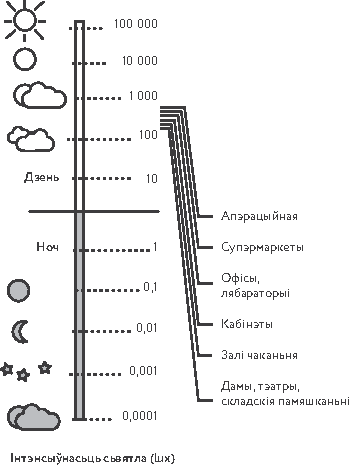
\includegraphics[scale=1.3]{willpower/ch12/1.pdf}
\end{figure}

У адным з~дасьледаваньняў было паказана, што ультрафіялет зьніжае атлусьценьне і прыкметы мэтабалічнага сындрому незалежна ад вітаміну D. У экспэрымэнце працяглае субэрытэмнае апраменьваньне ультрафіялетам прыводзіла да зьніжэньня вагі, паляпшэньня глюкозаталерантнасьці, павышэньня адчувальнасьці да інсуліну, зьмяншэньня прыкметаў тлушчавага гепатозу печані, зьніжэньня узроўняў нашчавага інсуліну, глюкозы і халестэрыну. Аўтары падкрэсьліваюць, што большасьць станоўчых эфэктаў сьвятла не аднаўлялася дадаткамі вітаміну D.

\subsection*{Пытаньні і заданьні}

1. Ці любіце вы бываць на сонцы?

2. Ці ведаеце вы свой узровень вітаміну D?

3. Якія з~вашых хатніх або рабочых справаў можна рабіць па-за домам?


\section{Як сонца ўплывае на здароўе?}

Сонца~--- адзін з~найважнейшых чыньнікаў здароўя і добрага самаадчуваньня. Дэфіцыт сонечнага сьвятла нэгатыўна адбіваецца на самых розных сыстэмах і органах: расьце рызыка атлусьценьня, дыябэту, сардэчна-сасудзістых і аўтаімунных захворваньняў, шэрагу відаў раку, пагаршаецца сон, павялічваецца рызыка дэпрэсіі, зьніжаецца лібіда. Вельмі небясьпечны дэфіцыт вітаміну D для цяжарных і дзяцей.

\textbf{Устаноўлена, што дастатковая колькасьць сонца зьніжае рызыку лімфомаў, раку грудзей, кішачніка, яечнікаў, падкарэньніцы, мачавога пухіра, стрававода, падстраўніцы, прамой кішкі, страўніка.}

\textbf{Правіла 1000 гадзінаў}~--- менавіта столькі часу нам трэба праводзіць на адкрытым паветры для забесьпячэньня аптымальнага здароўя, гэта каля трох гадзінаў на дзень. Вядома, правіла лягчэй выконваць, калі вы жывяце ў~сваім доме ці ў~вас ёсьць тэрасы і зручныя гаўбцы, дзе вы можаце прымаць ежу, працаваць і знаходзіцца на паветры.

\textbf{Сынхранізацыя біярытмаў.} Дастатковая колькасьць сонечнага сьвятла патрэбная для правільнай працы нашага ўнутранага гадзіньніка~--- супрахіязматычнага ядра. Сонечнае сьвятло прыкладна ў~30 разоў ярчэйшае за асьвятленьне ў~памяшканьнях, яно павялічвае ўзровень сератаніну, паляпшае сон, сынхранізуе біярытмы, паляпшае сакрэцыю мэлятаніну ўвечары, павялічвае якасьць сну, зьніжае рызыку дэпрэсіі і яшчэ шмат іншых аспэктаў. Сонечнае сьвятло ўяўляе сабой хвалі рознай даўжыні і інтэнсіўнасьці, у~якіх ёсьць розныя мэханізмы ўплыву. Карыснай зьяўляецца і яркасьць сьвятла бачнага спэктру: ультрафіялет А і ультрафіялет В маюць свае станоўчыя ўласьцівасьці, інфрачырвоны спэктр таксама валодае дабратворным эфэктам.

Самы просты спосаб палепшыць працу сваіх цыркадных гадзіньнікаў і біярытмаў~--- павялічыць колькасьць сьвятла днём. Гэта і лямпы фотатэрапіі, і простая рада «часьцей бываць на вуліцы». Але важна ня проста зрабіць «ярчэйшыя дні»: трэба яшчэ і зрабіць «ночы цямнейшымі», для мозгу важная менавіта гэтая розьніца. Для прыкладу, перапад дзённай і начной асьветленасьці для амішаў у~10 разоў больш, чым для сучаснага амерыканца. Можна пайсьці ў~турыстычны паход на прыроду. Дасьледаваньне паказала, што ўсяго два дні на прыродзе нармалізуюць цыркадныя рытмы, і ў~чалавека мэлятанін пачынае ўзрастаць вечарам на 1,4 гадзіны раней, чым да паходу.

\textbf{Сінтэз вітаміну D.} Сонечнае сьвятло спрыяе ўтварэньню вітаміну D. Яго колькасьць залежыць ад геаграфічнай шыраты, воблачнасьці, паравіны году, часу содняўк. Чым сьвятлейшая скура і больш адкрытых участкаў, тым больш утворыцца вітаміну D. Мае значэньне і час содняў~--- калі цень карацейшы за рост, то скура атрымлівае больш сонца, а~вось раніцай перад працай або позьнім вечарам пасьля выпрацоўка вітаміну D мінімальная. На жаль, гарадзкія жыхары бываюць на сонцы менавіта ў~той час, калі «цень даўжэйшы за рост», і вітамін D не выпрацоўваецца. Адзеньне, загар, узрост, смуга, забруджваньне паветра~--- усё гэта зьніжае выпрацоўку вітаміну D.

\emph{З 20 да 70 гадоў сінтэз вітаміну D у~скуры падае ў~4 разы. У людзей з~залішняй вагой тлушчавая тканіна актыўна паглынае вітамін D. У Дэлі дэфіцыт вітаміну D адчувае да 90\,\% жыхароў, і нават Аўстралія так заўзята змагалася з~ракам скуры, што атрымала дэфіцыт вітаміну D.} 

\textbf{Колькі ж вітаміну D выпрацоўваецца на сонцы?} Для разьліку выкарыстоўваецца складаная формула з~улікам вашага тыпу скуры, вагі, росту, месца пражываньня. Таму лепш скарыстацца праграмамі: Dminder (Android iOS) або SunDay: Vitamin D \& UV Monitor. Яны яшчэ і разьлічваюць бясьпечную для скуры колькасьць сонца для вашай геаграфіі і надвор'я. Калі я ў~плаўках выйду ў~Тайландзе ў~13:00 на пляж бяз крэму (чаго я, вядома, не раблю), то літаральна за 10 хвілін атрымаю 10.000 МЕ вітаміну D. 

\infobox{З дапамогай сонечных ваннаў можна стварыць у~падскурнай клятчатцы вялікі запас вітаміну D, якога хопіць і на зімовыя месяцы. Але лепш не рызыкаваць~--- і зімой прымаць прафіляктычныя дозы вітаміну.} 

Выпрацоўка вітаміну D адбываецца ў~скуры, ён утвараецца з~7-дэгідрахалестэролу пры ўзьдзеяньні ультрафіялету B (даўжыня хвалі 315--280 нм). Рэцэптары да вітаміну D ёсьць практычна ўсюды, таму вітамін D нават завуць гармонам. Ён рэгулюе ня толькі абмен кальцыя, але і ўплывае на рост клетак, сасудаў, выпрацоўку інсуліну, працу імуннай сыстэмы, палавой сыстэмы, актывуе транскрыпцыю каля 200 генаў.

\emph{Колькасьць атрыманага ўльтрафіялету вымяраюць у~мінімальных эрытэмных дозах, то бок яго колькасьці, неабходнай для ледзь прыкметнага пачырваненьня скуры. У год для падтрыманьня ўзроўню вітаміну D дастаткова ўсяго 50--60 эрытэмных дозаў. 1 эрітемной доза = 25.000 МЕ вітаміну D. Мінімум сонца~--- гэта чвэрць эрытэмнай дозы: ад 5 да 30 хвілін у~залежнасьці ад геаграфіі, 6--7 раз у~тыдзень на твар, рукі, ногі, з~10:00 да 15:00 у~сярэдніх шыротах.}

Як бачыце, для атрыманьня вітаміну D згараць зусім неабавязкова. Праўда, з~сонцам у~зімовыя месяцы будзе крыху цяжкавата.

\begin{figure}[htb!]
  \centering
  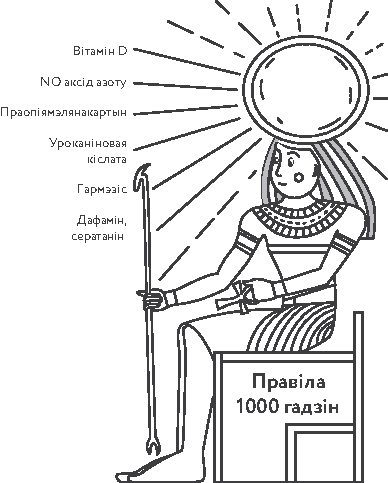
\includegraphics[scale=1.2]{willpower/ch12/2.pdf}
\end{figure}

\textbf{Дадаткі вітаміну D.} Калі ваш узровень вітаміну D ніжэй за 30 НГ / мл і вы ня можаце атрымаць дастатковую колькасьць сонца, то ёсьць сэнс прымаць яго дабаўкі. Для прафіляктыкі гіпавітамінозу D у~зімовы час, магчыма, таксама варта ўжываць яго ў~дадатках (але ня больш за 2000 МЕ у~дзень) і хаця б раз у~год вымяраць яго ўзровень у~плазьме крыві. Вітамін D, выпрацаваны ў~скуры, не распадаецца прынамсі ўдвая даўжэй, чым вітамін D у~дадатках. Перадазіроўка вітаміну D за кошт сонечных прамянёў немагчымая. Акрамя сонца і дабавак, невялікія колькасьці вітаміну D можна атрымліваць з~тлустай марской рыбай. Фізычная актыўнасьць павялічвае мабілізацыю вітаміну D з~тлушчу. Але сонца~--- гэта нашмат больш, чым вітамін D. І замяніць сонца дадаткам немагчыма. Давайце разьбяромся, якія ж ключавыя мэханізмы карыснага дзеяньня сонца.

\textbf{Сынтэз NO (аксід азоту).} Выбіраючыся на пікнік, гараджане часта заўважаюць, што ў~іх ад чыстага паветра ледзь ня кружыцца галава. Насамрэч гэта дзеяньне сонца.

\emph{\textbf{Можна правесьці навуковы экспэрымэнт}: для яго нам патрэбны таномэтр і 20-хвіліннае знаходжаньне на сонцы. Вымярыўшы ціск да і пасьля, вы зможаце ўбачыць, што ціск пасьля знаходжаньня на сонцы зьнізілася. Пад узьдзеяньнем сонца ў~сасудах выдзяляецца аксід азоту, які валодае сасудапашыральным дзеяньнем і абараняе ад атэрасклерозу.}

Аксід азоту~--- гэта актыўнае злучэньне, якое выпрацоўваецца ў~нашым арганізьме і валодае дабратворным узьдзеяньнем на здароўе сасудаў, пашыраючы іх, яно зьніжае запаленьне, паляпшае гаеньне ранаў, паляпшае працу мітахондрыяў, зьніжае рызыкі сардэчна-сасудзістых захворваньняў, узмацняе эрэкцыю і да т.~п. У нашай скуры захоўваецца шмат азоту ў~выглядзе нітратаў, нітрытаў і нітразатыёлу. Калі на скуру трапляе сонечнае сьвятло, адбываецца выпрацоўка аксіду азоту. Цікава, што для гэтага патрабуецца даўгахвалевы ультрафіялет А (315--400 нм), які менш расьсейваецца. Таму шпацыр на сонцы будзе карысны, нават калі вітамін D амаль не выпрацоўваецца. Фізычная актыўнасьць таксама дапамагае выдзяляцца аксіду азоту ў~сасудах, так што трэніроўка на адкрытым паветры пры сьвятле дня дае аптымальны эфэкт. Варта ўжываць у~ежу дастатковую колькасьць гародніны, дзе шмат карыснага азоту, напрыклад, чырвоны бурак.

\textbf{Зімовы сардэчна-сасудзісты фэномэн}~--- гэта пачашчэньне многіх хваробаў, ад трамбозаў да інсультаў, так зімой частата тромбаэмбаліі вышэй на 20\,\%, інсультаў~--- на 48\,\%, чым у~іншыя месяцы. Узімку вышэй узровень адрэналіну, ангіятэнзіну, гэтую зьяву тлумачаць і меншай рухомасьцю, і брудным паветрам, але ня будзем забываць пра наймацнейшы дэфіцыт~--- пра сонца. Сонца зьніжае рызыку сардэчна-сасудзістых захворваньняў рознымі спосабамі. Мы казалі пра вызваленьне аксіду азоту пад узьдзеяньнем ультрафіялету, але навукоўцы дасьледавалі і іншы мэханізм~--- яркасьць сьвятла.

\emph{Аказваецца, сьвятло сілай у~10\,000 люкс павялічвае актыўнасьць экспрэсіі цыркаднага гена Period 2 (PER2), што ў~сваю чаргу павялічвае актыўнасьць гіпаксіяй індукаванага фактару HIF1A. А HIF1A у~сваю чаргу аказвае ахоўны эфэкт у~розных тканках.}

\infobox{Такім чынам, яркае сьвятло абараняе ад сардэчна-сасудзістых захворваньняў і, у~выпадку інфаркту, значна абмяжоўвае пашкоджаньне сардэчнай мышцы.}

\textbf{Праопіямэлянакартын}~--- гэта гіпафізарны прагармон, пад узьдзеяньнем сонца яго выпрацоўка павялічваецца. Сам па сабе ён неактыўны, але разразаецца спэцыфічнымі фэрмэнтамі эндапэптыдазамі трыма спосабамі, даючы розныя мэтабаліты: ліпатрапін (гармон тлушчаспаленьня), эндарфіны (задавальненьне), мэлянацытстымулёўны гармон (колер скуры), адрэнакартыкатропны гармон (стрэс).

\emph{У экспэрымэнтах увядзеньне мэлянакартынаў памяншала колькасьць зьяданай ежы і спрыяла пахудзеньню. Таму павелічэньне часу знаходжаньня на сонцы дапаможа вам зьменшыць вагу. А вось адсутнасьць сонца зьмяншае спальваньне тлушчу, магчыма, гэтая рэакцыя зьяўляецца эвалюцыйна набытай для выжываньня зімой, калі мала ежы. Акрамя гэтага, мэлянацытстымулёўныя гармоны зьніжаюць узровень хранічнага запаленьня, палягчаючы цячэньне шматлікіх захворваньняў.} 

\textbf{Ураканінавая кіслата.} Пад узьдзеяньнем ультрафіялету В разам з~утварэньнем вітаміну D адбываюцца і зьмены ўраканінавай кіслаты. Пры трапленьні сонца на скуру яе транс-форма ператвараецца ў~цыс-форму з~паглынаньнем вялікай колькасьці энэргіі. У цемры ж назіраецца зваротны працэс: яна мяняе канфігурацыю, расьсейваючы назапашаную энэргію ў~выглядзе цяпла. Гэты мэханізм нараўне з~утварэньнем мэляніну абараняе клеткі скуры ад пашкоджаньня. Цікава, што ўраканінавая кіслата выдзяляецца з~потам, забясьпечваючы абарону на паверхні скуры. Таму пры моцным ветры згарэць можна хутчэй. Карысьць ураканінавай кіслаты ня толькі ў~абароне скуры. Пры ўзьдзеяньні сонца яе ўзровень павялічваецца і ў~мозгу, дзе яна зьяўляецца пры ператварэньні амінакіслоты гістыдзіну ў~глутамінавую кіслату. Глутамат~--- гэта адзін з~галоўных узбуджальных нэўрамэдыятараў мозгу. У дасьледаваньнях у~жывёлаў пасьля апрамяненьня ультрафіялетам паляпшаліся кагнітыўныя функцыі. 

Ураканінавая кіслата~--- чыньнік стрымліваньня актыўнасьці імуннай сыстэмы: пры яе недахопе павялічваюцца рызыкі алергічных і аўтаімунных захворваньняў, а~вось пры лішку можа ўзьнікаць імунасупрэсія. 

\textbf{Рэтынальны дафамінавы шлях.} Сонечнае сьвятло павышае ўзровень дафаміну ў~мозгу~--- гэта зьвязана з~шэрагам дафамінавых эфэктаў, ад павышэньня ўзроўню энэргіі да паляпшэньня адчувальнасьці да інсуліну. Памятайце пра тое, што паўсюдна насіць сонцаахоўныя акуляры~--- гэта не заўсёды здаровы выбар! Рэч у~тым, што ў~сятчатцы вока ёсьць асаблівая рэтынальная дафамінавая сыстэма, зьвязаная з~мозгам.

\textbf{Таму сонца напрамую можа павысіць вам дафамін. А абараніць сятчатку ад ультрафіялету вы можаце харчовым спосабам: сятчатка мае патрэбу ў~высокіх канцэнтрацыях лютэіну, зэаксантыну і Амэга-3.}

\subsection*{Пытаньні і заданьні}

1. Ці лепш вы сьпіце, калі правялі больш часу на адкрытым паветры?

2. Ці ёсьць у~вас магчымасьць сярод працоўнага дня бываць на гаўбцы, тэрасе ці выходзіць на вуліцу?

3. Як адрозьніваецца ваша самаадчуваньне ў~сонечныя і пахмурныя дні? А ўлетку і ўзімку?


\section{Правільна выкарыстоўвайце сонца}

У сонечнага сьвятла, як і ў~любога іншага эфэктыўнага сродка, ёсьць пабочныя эфэкты. Таму важна бываць на адкрытым паветры, але ня менш важна пазьбягаць залішняга ультрафіялету (УФ).

\emph{Бываючы ў~адпачынку, я заўсёды дзіўлюся бестурботнаму стаўленьню да сонца: калі мы вяртаемся з~мора аб 11-й раніцы, шмат хто толькі ідзе загараць. А калі мы зноў ідзём на мора ў~16:00, людзі толькі вяртаюцца. Вядома, загараць у~самы небясьпечны час~--- шкодна.}

Лішак сонечнага сьвятла прыводзіць да паскоранага фотастарэньня скуры, павялічвае рызыку раку скуры, зьяўленьня пігмэнтных плямаў, разьвіцьця дыстрафіі сятчаткі вачэй. Таксама не рэкамэндую загараць у~салярыі. Небясьпека загару яшчэ і ў~тым, што пашкоджаньні скуры назапашваюцца паступова, пачынаючы з~самага дзяцінства, і выяўляюцца пры старэньні. Дасьледаваня блізьнятаў паказалі вырашальны ўплыў ультрафіялету на старэньне скуры.

\textbf{Пазьбягайце небясьпечнага часу.} У гарачых краінах найбольш небясьпечныя гадзіны з~высокім УФ індэксам~--- з~11.30 да 15.30, а~пры вельмі высокім~--- з~10:00 да 17:00. У гэты час варта мінімізаваць знаходжаньне на сонцы або выкарыстоўваць шыракаполы капялюш і насіць адзеньне з~доўгімі рукавамі. Не забывайце, што на нас падае ня толькі прамое, але і адлюстраванае сьвятло, і можна згарэць, расслабляючыся пад парасонам. Калі вы бачыце шмат неба, то, нават знаходзячыся ў~цені, атрымліваеце вялікую дозу ультрафіялету. Пры вельмі яркім сонца носіце сонцаахоўныя акуляры з~УФ-фільтрам, гэта зьнізіць рызыку катаракты і захворваньняў сятчаткі вачэй.

\textbf{Важна пазьбягаць залішняга ультрафіялету, бо пашкоджаньні скуры назапашваюцца паступова і могуць выявіцца толькі ў~старасьці.}

У прагнозе надвор'я паказваюць \textbf{ультрафіялетавы індэкс}, больш высокія значэньні якога небясьпечныя сонечнымі апёкамі і пашкоджаньнем скуры і вачэй. На колькасьць ультрафіялету ўплываюць розныя фактары: воблачнасьць, смуга, таўшчыня азонавага пласта (чым ён танчэйшы, тым больш ультрафіялету пранікае). Чым вышэй індэкс, тым менш варта быць на сонца.

\begin{figure}[htb!]
  \centering
  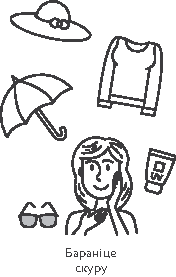
\includegraphics[scale=1.5]{willpower/ch12/3.pdf}
\end{figure}

\textbf{Паступова павялічвайце час знаходжаньня на сонцы.} Не загарайце падоўгу, асабліва калі да гэтага вы доўга не былі на сонцы. Патроху і плыўна павялічвайце працягласьць сонечных ваннаў. Рэзка згарэць, прыехаўшы ў~адпачынак,~--- гэта вельмі шкодна для скуры і здароўя ў~цэлым. Сонечныя апёкі павялічваюць рызыку мэляномы скуры ў~два разы. Рэгулярная гадзіна загару ў~дзень~--- для пачатку цалкам дастаткова, а~ў гарачых краінах вам хопіць і паўгадзіны.

\textbf{Сонцаахоўны крэм} з~высокім значэньнем зьяўляецца добрай абаронай ад сонца. Але я ўсё ж раю выбіраць аптымальны час і скарачаць знаходжаньне на сонцы, чым ляжаць на сонцапёку, абмазаўшыся крэмам. Дасьледаваньні паказваюць, што ў~людзей, якія часта выкарыстоўваюць крэм з~SPF, вышэйшая рызыка раку скуры. Гэта адбываецца таму, што крэм дае ілюзію поўнай засьцярогі ад сонца. Людзі наносяць менш, чым трэба, крэм змываецца вадой.

\emph{Магчыма ёсьць і іншы мэханізм: большасьць ахоўных чыньнікаў паглынаюць толькі ультрафіялет В, які выклікае апёкі. Але пры гэтым парушаецца мэханізм абароны скуры ад загару ў~цэлым, што дазваляе ультрафіялету А пранікаць у~высокіх дозах. Таксама выказваюцца асьцярогі, што кампанэнты крэму пад дзеяньнем сонца могуць утвараць таксічныя рэчывы, якія пры гэтым лёгка ўсмоктваюцца ў~скуру.}

\textbf{Рызыка раку скуры.} Калі вы рэгулярна бываеце на сонцы, то рызыка мэляномы скарачаецца на 14\,\%. Згодна з~дасьледаваньнем сярод маракоў флоту ЗША, верагоднасьць разьвіцьця мэляномы на 34\,\% вышэй у~тых, хто служыць у~труме. Рызыка раку мэляномы павялічваецца, калі яна ёсьць у~вашых сваякоў, пэрсаналізаваць рызыку можна і па ДНК-тэсце. Рэгулярна аглядайце свае радзімкі самі ці ў~дэрматоляга, можна скласьці адмысловую «мапу цела». Пры гэтым колькасьць радзімак не зьвязаная з~рызыкай мэляномы. Ёсьць спэцыяльныя праграмыі для тэлефона, якія могуць аналізаваць фота радзімак.

\emph{\textbf{Правіла ABCDE}: Asymmetry, Border, Color, Diameter, Evolution: асімэтрыя радзімкі, няроўны ці невыразны контур, неаднародны ці незвычайны колер, вялікі дыямэтр і заўважная зьмена прыкметаў, у~т.л. сьверб,~--- гэтыя прыкметы не залежаць адна ад аднае, таму кансультуйцеся ў~лекара, нават калі заўважылі адну зь іх!}

Абараняйце радзімкі ад сьвятла, беражыце іх ад траўмаваньня рамянямі, абуткам, бюстгальтарам. Пазьбягайце салярыю і сонечных апёкаў. Выдаляючы падазроныя радзімкі, абавязкова трэба праводзіць іх гісталягічнае вывучэньне.

\textbf{Каратыноіды.} Калі чалавек есьць мала гародніны, то ўзімку, а~часам і ўлетку, будзе ``нездарова'' бледным. Як вядома, колер скуры вызначаецца пераважна трыма пігмэнтамі: гемаглабінам, мэлянінам і каратыноідамі (выключаючы іншыя, рэдкія або паталягічныя пігмэнты). Каратыноіды~--- адны з~маіх любімых злучэньняў, да іх адносяцца бэта-каратын, лікапін, альфа-каратын і ксантафілы, такія як лютэін і зэаксантыін. Каратыноіды граюць важную ролю ў~самых разнастайных працэсах, ад зьяўленьня сардэчна-сасудзістых захворваньняў і ўплыву на працягласьць жыцьця да разьвіцьця катаракты і ўмацаваньня фотаабароны. Фотастарэньне скуры~--- важная праблема, плюс каратыноіды~--- гэта тлушчараспушчальныя злучэньні, таму яны добра працуюць і ў~скуры, і ў~тлушчавай тканцы, і ў~галаўным мозгу.

\emph{Напрыклад, лютэін абараняе ў~мозгу і сятчатцы Амэга-3 тлустую ДГК ад акісьленьня.} 

Каратыноіды ўбудоўваюцца ў~нашы клеткавыя мэмбраны і абараняюць іх ад пашкоджаньняў свабоднымі радыкаламі, а~таксама цэласнасьць клетак і тканін ад ультрафіялету і ня толькі. Калі такі фізычны мэханізм не спрацаваў, то каратыноіды могуць проста прымаць удар на сябе, акісьляючыся. Агляд дасьледаваньняў пацьвярджае, што людзі, якія ўжываюць дастаткова садавіны і гародніны, багатых каратыноідамі (морква, памідоры, папая), маюць менш паталёгіяў скуры, і іх скура пад дзеяньнем ультрафіялету павольней старэе.

\emph{Так, умераная доза бэта-каратыну зьмяншае рэакцыю скуры на дзеяньне ўльтрафіялету. У адным дасьледаваньні параўноўвалі дзеяньне таматнага соку, экстракту тамата і сынтэтычнага лікапэну. Максімум утрыманьня іх у~скуры назіраўся праз 12 тыдняў~--- гэта зьвязана з~хуткасьцю абнаўленьня скуры і кумуляцыі лікапэну. Пры гэтым экстракт тамата на 48\,\% павялічыў фотаабарону, а~вось дадатак лікапэну~--- на 25\,\%. Вось відавочная карысьць цэльнай гародніны, у~якой утрымоўваецца цэлы шэраг фотапратэктараў, такіх як фітафлуен, фітаен і інш.}

Акрамя гародніны, эфэктыўным для фотаабароны можа быць прыём астаксанцыну ў~выглядзе дадаткаў. Толькі пачаць яго прыём трэба за 1--2 месяцы да паездкі ў~гарачыя краіны, каб ён пасьпеў назапасіцца ў~скуры. Фотаахоўнымі ўласьцівасьцямі таксама валодае какава.

\textbf{Фотасэнсібілізатары.} Будзьце асьцярожныя з~сонцам, калі прымаеце лекі, якія валодаюць уласьцівасьцямі фотасэнсібілізатараў: сульфаніламіды, тэтрацыкліны, фэнатыязіны, фторхіналоны, нестэроідныя супрацьзапаленчыя прэпараты, некаторыя гарманальныя прэпараты, некаторыя віды касмэтыкі~--- з~дадаткамі вітамінаў, рэтынавай кіслаты, этэрных алеяў і г.~д..

\emph{\textbf{Фотаадчувальнасьць.} Грэйпфрут зьмяшчае фуранакумарыны (псарален), якія ўзмацняюць адчувальнасьць да ультрафіялету. Як і іншыя цытрусавыя, яго штодзённае ўжываньне павялічвае рызыку мэляномы. Так, штодзённае спажываньне 1,6 порцыі цытрусавых павышае рызыку мэляномы на 36\,\%.} 

Фотасэнсібілізатары ўваходзяць і ў~склад некаторых расьлінаў, напрыклад сьвятаяньніка: у~ім утрымліваюцца гіпэрыцын і псэўдагіпэрыцын, якія могуць выпрацоўваць актыўныя формы кіслароду ў~прысутнасьці сонца. Таму сьвятаяньнік, асабліва ў~фотаадчувальных людзей, можа выклікаць сонечныя апёкі.

\subsection*{Пытаньні і заданьні}

1. Ці бледная ў~вас скура? Дадайце больш гародніны ў~свой рацыён!

2. Ці выконваеце вы правілы бясьпекі на сонца?

3. Вывучыце свае радзімкі і складзіце ``мапу скуры''.


\section{Тэмпэратурнае забруджваньне}

Калі мы глядзім на сябе ў~люстэрка, то, апроч іншага, бачым вынік уплыву тэмпэратуры на наш выгляд: валасы ў~нас растуць у~асноўным толькі на галаве, і ня надта інтэнсіўна~--- на целе. Зразумець, калі продкі чалавека пачалі губляць валасы, цяжка, бо парэшткі не даюць на гэта адказу. На дапамогу прыходзіць вывучэньне ДНК вошай, якія жывуць на галаве і ў~лабковых валасах. Верагодна, 2 мільёны гадоў таму валасы расьлі ўжо не на ўсім целе, а~200 тысячаў гадоў таму нашы продкі сталі насіць адзеньне. Чалавека часам завуць ``безвалосай малпай'', але пры гэтым забываюць пра прычыны, якія прывялі да гладкай скуры.

\subsection*{Прыстасаваньне да высокіх тэмпэратураў}

Адна з~тэорый эвалюцыі вястуе: нашы продкі пазбавіліся большай часткі валасоў, каб павысіць эфэктыўнасьць тэрмарэгуляцыі. Вымушана пакінуўшы лес, яны апынуліся пад пякучым сонцам саваны. Вядома, яны ўжо хадзілі на дзьвюх нагах, і гэта дапамагала не перагравацца, бо сумарнае цеплавое ўзьдзеяньне ніжэйшае, калі стаіш. А калі бяжыш, дык яшчэ і ахалоджваесься ветрам. Але нават двухногаму цяжка доўга бегчы на сьпякоце~--- літаральна праз паўгадзіны ён бы пераграваўся і рабіўся здабычай драпежнікаў. Страта валасоў і пяціразовае павелічэньне колькасьці потавых залозаў павысілі эфэктыўнасьць тэрмарэгуляцыі. Гэта забясьпечыла чалавеку дзівосныя магчымасьці і зрабіла яго істотай, якая можа бегчы даўжэй за ўсіх і на вялікіх адлегласьцях абагнаць нават каня.

\emph{Так, чалавек бяжыць павольна, але можа бегчы доўга, і маратонцы гэта пацьвярджаюць. Напрыклад, гепард, хоць ён і самы хуткі, ня можа бегчы дыстанцыі больш за 1 кілямэтр, бо пераграваецца. Навукоўцы назіралі, як бушмены ў~40-градусную сьпякоту заганяюць антылопу: палохаюць і гоняцца за ёй па сьлядах, не даючы адпачыць і астыць, пакуль яна не падае праз перагрэў.}

Ёсьць меркаваньне, што нават аблысеньне ў~мужчынаў зьяўляецца адаптацыяй для лепшага астываньня~--- бо на галаве шмат капіляраў. Па меры росту вусоў і барады плошча для астуджэньня памяншаецца, і прырода кампэнсуе гэта павелічэньнем паверхні голай скуры на макаўцы.

\subsection*{Прыстасаваньне да нізкіх тэмпэратураў}

Каля 65 мільёнаў гадоў таму ў~раёне паўвострава Юкатан упаў вялізны мэтэарыт. Яго падзеньне падняло ў~паветра багацьце пылу, які не асядаў гадамі. ``Ядзерная зіма'' прывяла да выміраньня дыназаўраў і хуткай эвалюцыі млекакормячых. Адным з~мэханізмаў, які дазволіў нашым продкам дамінаваць, быў разьвіты тэрмагенэз (цеплаўтварэньне)~--- здольнасьць цела падтрымліваць пастаянную тэмпэратуру. Так яны атрымалі перавагу ў~эвалюцыйнай гонцы.

Некаторыя мэханізмы адаптацыі~--- ужо неэфэктыўныя рудымэнты, напрыклад, гусіная скура. Мурашкі~--- гэта скарачэньне маленькіх цягліцаў у~скуры, якія павінны падымаць валасы пры холадзе (вышэйшы валасяны полаг~--- больш паветра як уцяпляльніка) або агрэсіі (для візуальнага павелічэньня памераў), але валасоў, на жаль, ужо няма.

\emph{Некаторыя людзі, напрыклад, «Ледзяны чалавек» Вім Хоф, паказваюць дзівосныя магчымасьці чалавечага цела. Але нічога экстраардынарнага ў~гэтым няма, гэтаму можна навучыцца і да шмат чаго звыкнуць: якуты вунь шаруюць нованароджаных сьнегам.}

Людзі маюць прыродную ўстойлівасьць да нізкіх тэмпэратураў і множныя мэханізмы адаптацыі. Рэакцыя на цяпло і холад шмат у~чым залежыць ад функцый шчытавіцы, таму пры непераноснасьці высокіх і нізкіх тэмпэратураў важна праверыць яе працу.

Вылучаюць два спосабы цеплаўтварэньня: скарачальны тэрмагенэз: калоціць, дрыжыць, «зуб зуба паганяе», пры якім цеплаўтварэньне абумоўлена скарачэньнямі шкілетных цягліц (прыватны выпадак~--- халадовая цяглічная дрыготка); нескарачальны тэрмагенэз~--- праца бурай тлушчавай тканкі.

Пры дрыготцы выпрацоўка цяпла ўзрастае больш чым у~тры разы, а~пры інтэнсіўнай фізычнай працы~--- у~дзесяць і болей разоў.

\begin{figure}[htb!]
  \centering
  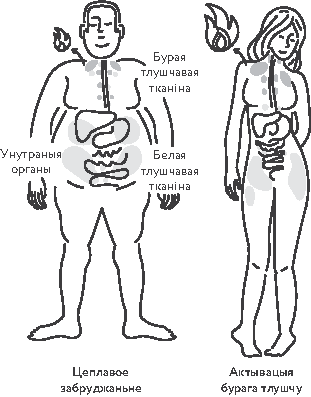
\includegraphics[scale=1.5]{willpower/ch12/4.pdf}
\end{figure}

Разумовая і фізычная актыўнасьць павялічваюцца пры павышэньні тэмпэратуры цела і зьмяншаюцца, калі халодна. Спартоўцы ведаюць, што «разаграваньне» павышае вынікі, а~навукоўцы ўсталявалі, што інтэнсіўныя прысяданьні могуць узбадзёрыць ня горш за кафэін. Пры захворваньні арганізм сам павышае тэмпэратуру, каб больш эфэктыўна змагацца з~хваробай: калі вы будзеце зьбіваць тэмпэратуру, калі яна павышана нязначна і нармальна пераносіцца, гэта перашкодзіць нармальнаму імуннаму адказу!

\emph{Аказваецца, нэўроны ў~дугападобным ядры гіпаталямуса, якія рэгулююць апэтыт, адчувальныя і да ваганьняў тэмпэратуры цела. Таму фізычная актыўнасьць, якая падвышае тэмпэратуру цела, ня толькі спальвае калёрыі, але і дапамагае паменшыць голад. А ляжаньне на канапе можа толькі ўзмацніць цягу да ежы. Гэтыя ж нэўроны экспрэсуюць праопіямэлянакартын, таму апэтыт памяншаецца і пры павелічэньні знаходжаньня на сонца, і пры выпрацоўцы эндарфінаў (радасьць, лазня, сэкс і да т.~п.). Таксама на гэтых нэўронах ёсьць адмысловыя тжрмаадчувальныя рэцэптары, якія могуць быць актываваныя рэчывамі, што пакідаюць адчуваньне халоднае (ментол, мята, эўкаліпт) або гарачае (імбір, гваздзік, хрэн, чырвоны перац). Яны таксама стымулююць тлушчаспаленьне і прыгнятаюць апэтыт.}

\subsection*{Цеплавое забруджваньне}

Цікава, што мы з~вамі мярзьлівейшыя за сваіх продкаў. Яшчэ 150 гадоў таму нармальная тэмпэратура цела была роўна 37°С, а~сёньня сярэднія значэньні дасягаюць 36,4°С. Сярод прычын гэтага абмяркоўваецца як зьніжэньне колькасьці інфэкцыяў, так і зьніжэньне базавага абмену празь нізкую фізычную актыўнасьць, зьніжэньне тэрмагенэзу праз знаходжаньне ў~пастаянным цеплавым камфорце. Калі раней наш арганізм адаптаваўся для барацьбы зь пераахаладжэньнем, то цяпер нам пагражае пераграваньне.

Сёньня ў~нас зьявілася цёплае адзеньне, мы жывём у~цёплых дамах. Людзі імкнуцца зрабіць сваё жыцьцё гарачэйшым, бо «ад цяплосьці не баляць косьці». Але лішак цяпла шкодзіць здароўю і мае назву ``цеплавое забруджваньне''. Тэрмастабільнасьць на працягу ўсяго жыцьця дэтрэніруе сыстэмы тэрмарэгуляцыі і мэтабалізму. Чым вышэй тэмпэратура вакол нас, тым вышэй рызыкі парушэньня абмену рэчываў. Навукоўцы ўстанавілі, што павышэньне сярэдняй тэмпэратуры на адзін градус у~год можа выклікаць тысячы выпадкаў захворваньня на дыябэт. Бо ў~пастаянным цяпле зьніжаецца актыўнасьць бурага тлушчу і адчувальнасьць да інсуліну.

Здаровы тэмпэратурны рэжым дапамагае нам ня толькі мацней спаць, лепш выглядаць, але і падвышае разумовую і фізычную актыўнасьць~--- аж да падаўжэньні жыцьця. Сыстэмы астуджэньня вельмі важныя, у~т.л. і для працы мозгу. Тэмпэратура мозгу рэгулюе актыўнасьць нэрвовай тканкі, мо таму пра чалавека, які рацыянальна разважае, гавораць, што ў~яго ``халодная галава''.

\textbf{Буры тлушч} называецца так праз свой колер і выглядае так таму, што ў~клетках яго вельмі шмат мітахондрый з~асаблівым бялком тэрмагенінам (разьяднальны бялок). У бурым тлушчы актыўна ідуць працэсы акісьленьня тлушчаў, толькі ўтварааецца пры гэтым не энэргія для клеткі ў~выглядзе АТФ, а~цеплыня.

\textbf{За год 50 г бурага тлушчу могуць спаліць да 4--5 кг белага тлушчу.} Колькасьць бурага тлушчу рэзка зьніжаецца да 40 гадоў: звычайна ў~дарослага чалавека ёсьць усяго 20--30 грамаў актыўнага бурага тлушчу, у~асноўным у~надключычнай вобласьці. Выяўлена, што ў~людзей, якія маюць лішнюю вагу, колькасьць бурага тлушчу зьніжаная, а~яго актыўнасьць прыгнечаная. Пры пэўных умовах (меншая тэмпэратура паветра, вялікая фізычная актыўнасьць) частка клетак звычайнага ``белага'' тлушчу могуць пачаць паводзіць сябе як бурыя, тады іх называюць ``бэжавы тлушч''. Актывацыя бурага тлушчу паляпшае абмен рэчываў, абараняе ад дыябэту, паляпшае адчувальнасьць да інсуліну.

\textbf{Разьяднальныя бялкі (UCP)} знаходзяцца на мэмбране мітахондрый і спрыяюць таму, што назапашаная ў~выглядзе розьніцы патэнцыялаў энэргія сыходзіць у~цеплыню, г.~зн. разьядноўваюць акісьленьне і фасфараляваньне. Падобныя выдаткі аказваюцца вельмі карыснымі для арганізма.

\emph{Аказалася, што UCP-1 у~бурай тлушчавай тканцы спрыяе падтрыманьню нармальнай вагі (паляпшаючы адчувальнасьць да інсуліну, павялічваючы тлушчаспаленьне і інш.), UCP-2 у~гіпакампе паляпшае нэўрагенэз і нэўраплястычнасьць, а~ў гіпаталямусе~--- уплывае на агульны ўзровень мэтабалізму і падаўжае жыцьцё. UCP-2 таксама абараняе ад лішку актыўных формаў кіслароду (АФК), а~UCP-3 у~цягліцах паляпшае эфэктыўнасьць тлушчаспаленьня пры фізычнай актыўнасьці.}

Разьяднальныя бялкі ёсьць ня толькі ў~бурым і бэжавым тлушчы, іх шмат у~печані, у~цягліцах, сэрцы і ў~іншых тканках. Холад, фізычная актыўнасьць, пэўны рэжым харчаваньня і прадукты~--- безь перакусаў і без высокавугляводаў ежы~--- павялічваюць колькасьць разьяднальных бялкоў. Навуковец Джон Спікмэн высунуў ідэю, што колькасьць разьяднальных бялкоў, якія зьніжаюць утварэньне актыўных формаў кіслароду, грае ключавую ролю ў~падаўжэньні жыцьця. Гэтая тэорыя таксама носіць назву ``разьяднай і выжывай'' (Uncoupling-to-Survive) і вястуе, што чым вышэй хуткасьць мэтабалізму і чым больш разьяднальных бялкоў, тым лепшая праца мітахондрый і большая працягласьць жыцьця.

\subsection*{Пытаньні і заданьні}

1. Як вы пераносіце холад і цяпло?

2. Якая тэмпэратура ў~вас дома ўдзень і ўначы? Усталюйце градусьнік, можна сынхранізаваны са смартфонам, каб вымяраць содневыя ваганьні.

3. Ці выкарыстоўваеце вы гострыя і пякучыя спэцыі?


\section{Халадовы і цеплавы пратакол}

Холад мае вялікую колькасьць станоўчых эфэктаў для здароўя: ён дапамагае зьнізіць вагу, павышае адчувальнасьць да інсуліну, нават паляпшае мікрафлёру, зьніжае рост пухлін, павышае імунітэт, аказвае супрацьзапаленчае ўзьдзеяньне, зьніжае акісьляльны стрэс, паляпшае стан касьцей. Таксама халадовыя працэдуры стымулююць выпрацоўку шэрагу карысных ахоўных малекул і актывуюць сыгнальныя шляхі (FGF-21, адыпанэктын, ірызын, SIRT1, бялкі цеплавога шоку).

\infobox{Холад абараняе мозг ад ішэмічных пашкоджаньняў, павялічвае фэртыльнасьць, паляпшае працу шчытавіцы.}

Цікава, што тыя жывёлы, якія ўпадаюць у~сьпячку, жывуць нашмат даўжэй за сваіх суродзічаў. Так, звычайная мыш жыве тры гады, а~кажан, які ўпадае ў~сьпячку больш чым на паўгода, дажывае да 18 гадоў!

\textbf{Гартаваньне} складаецца з~мноства розных мэтадаў, але варта праяўляць паступовасьць і бясьпеку ў~іх выкарыстаньні. Экстрэмальныя мэтады накшталт працяглага маржаваньня ў~ледзяной вадзе я ня раю, бо занадта моцны тэмпэратурны стрэс можа нанесьці шкоду. Пачынаць варта з~паветранага ахалоджаньня і затым пераходзіць да воднага, бо вада нашмат мацней адводзіць цеплыню.

У гэтай справе, як і ў~шматлікіх іншых, важныя правільны псыхалягічны настрой і ўпэўненасьць: гартуемся на мяжы задавальненьня, але не гвалтуем сябе. Пры працэдуры скура павінна чырванець: калі яна бляднее ці сінее, то нагрузка празьмерная. Калі адчуваеце, што замярзаеце, трэба неадкладна спыніць працэдуру і сагрэцца. Таксама важна выконваць адпаведную дыету і пазьбягаць абязводжваньня. Дадаткі Амэга-3, адаптагенаў дапамогуць лягчэй адаптавацца да холаду.

\textbf{Паветраныя ванны.} Апранайце менш лішняга адзеньня дома і на вуліцы: вы ідэальна апранутыя, калі вам халодна стаяць, але цёпла ісьці. Тэмпература 18--20 градусаў спрыяе падтрыманьню цяглічнага тонусу.

Вы можаце рабіць зарадку з~адкрытымі вокнамі і галяком~--- адсутнасьць адзеньня ўзмацняе цеплааддачу. Паводле словаў Уладзіміра Маякоўскага: ``Няма на сьвеце прыгажэйшага адзеньня, чым бронза мускулаў і сьвежасьць скуры''. Бэнджамін Франклін заўсёды пачынаў свае дні з~паветраных ваннаў: на працягу паўгадзіны кожны дзень ён сядзеў перад разнасцежаным акном галяком, чытаючы, робячы запісы, разважаючы. Сон у~прахалодзе паляпшае мэтабалічныя паказьнікі нават здаровых людзей: мерзнуць ня трэба, спіце пад коўдрай і ўдыхайце прахалоднае паветра.

Гартаваньне актыўна ўжываецца ў~шматлікіх дзіцячых садах, школах і выхаваўчых установах як сродак умацаваньня здароўя: носім шорты, прымаем халодны душ, пакідаем адкрытыя вокны ў~спальнях.

\emph{Дасьледаваньні паказалі, што тэмпэратура ў~доме 19 градусаў прыводзіць да павелічэньня актыўнасьці бурага тлушчу да 40\,\%, што спрыяе лепшаму абмену і пахудзеньню!}

\textbf{Лякальнае ахалоджаньне.} Галава, ручыцы і ступні маюць вялікую колькасьць халадовых рэцэптараў і граюць вельмі важную ролю ў~тэрмарэгуляцыі. Умываньне халоднай вадой, хаджэньнея басанож на прыродзе і дома, мыцьцё твару кубікам лёду~--- карысныя. Для трэніроўкі можна выкарыстоўваць апусканьне твару з~затрымкай дыханьня ў~ваду тэмпэратурай 10 градусаў.

\textbf{Агульнае ахалоджаньне.} Купаньне, плаваньне, кантрасны душ, халодны душ, абліваньні вадой карысныя для здароўя~--- гэта выдатныя варыянты карыснага стрэсу (гармэзісу), які ўмацоўвае нашу стрэсаўстойлівасьць! Некаторыя аўтары прапануюць выкарыстоўваць халодныя ванны, накладаньне лёду на цела, маржаваньне і да т.~п. Аднак злоўжываньне халадовымі працэдурамі нясе рызыкі для здароўя, у~тым ліку прыгнёт імунітэту, моцны стрэс, павышэньне рызыкі сардэчнага прыступу і да т.~п. Важна ўлічыць: працяглы моцны холад выклікае выкід эндарфінаў, таму некаторыя людзі падсаджваюцца на яго.

\emph{Акрамя хатніх спосабаў, актыўна выкарыстоўваюцца як касмэтычныя і аздараўленчыя працэдуры~--- крыяліполіз і крыясаўна.}

\textbf{Спорт.} Усе віды фізычнай актыўнасьці паляпшаюць працу бурага тлушчу і выдатна дапаўняюць халадовыя працэдуры. Прахалода падтрымлівае адэкватны цяглічны тонус, стымулюе актыўнасьць за кошт павышэньня адрэналіну і норадрэналіну. Трэніроўкі павялічваюць узровень гармону ірызіну (ген FNDC5), які стымулюе ператварэньне белага тлушчу ў~буры (бэжавы). Прасьцейшы і дзейсны пры гэтым варыянт~--- хуткая хадзьба ўвосень або ўзімку.

\infobox{Ідэальная раніца~--- гэта спорт на вуліцы ў~прахалодзе і нашча, каб стымуляваць тэрмагенэз.}

\textbf{Здаровае харчаваньне} выдатна спалучаецца з~гартаваньнем: важна мець у~рацыёне дастатковую колькасьць бялку і тлушчаў і выключыць высокаглікемічныя вугляводы: інсулін душыць працу бурага тлушчу. Умеранае абмежаваньне калярыйнасьці ежы прыводзіць да двухразовага павелічэньня экспрэсіі генаў UCP-2 і UCP-З у~адыпацытах і шкілетных цягліцах. Звужэньне харчовага акна, а~таксама ўмеранае абмежаваньне калярыйнасьці дапамагаюць павысіць тлушчаспаленьне. Павышаюць актыўнасьць бурага тлушчу аліўкавы алей і Амэга-3 тоўстыя кіслоты, розныя каратыноіды, напрыклад, фукаксантын з~марскіх водарасьцяў.

\textbf{Амэга-3} тлустыя кіслоты зьяўляюцца своеасаблівым клеткавым «антыфрызам», якія абараняюць мэмбраны ад замярзаньня. Менавіта таму рыбы, якія жывуць у~халодных ці глыбокіх морах, маюць максімальнае ўтрыманьне Амэга-3 тлустых кіслот, а~глябальнае пацяпленьне прыводзіць да зьніжэньня ўтрыманьня Амэга-3 у~рыбе.

\emph{Холад суправаджае Амэга-3 тлустыя кіслоты з~самага пачатку іх сынтэзу~--- іх вырабляюць асаблівыя дыятомавыя водарасьці, якія растуць у~халодных і чыстых водах. Сынтэзуюцца яны з~тае прычыны, што ў~холадзе трэба падтрымліваць аптымальную глейкасьць клеткавых мэмбранаў. А вось цёплыя і каламутныя воды пераважна насяляюць сіне-зялёныя водарасьці, якія не валодаюць такой здольнасьцю, вось чаму ў~рачной рыбе вельмі мала Амэга-3.}

Навуковыя дасьледаваньні паказваюць прыкметны ўплыў Амэга-3 на халадовую ўстойлівасьць, прычым адразу па некалькіх мэханізмах, уключаючы прамы ўплыў на бэжавы і буры тлушч. Амэга-3 зьвязваецца з~рэцэптарам GPR120, што прыводзіць да выдзяленьня гармону FGF21, які ўзмацняе выпрацоўку цяпла ў~тлушчавай тканцы.

\begin{figure}[htb!]
  \centering
  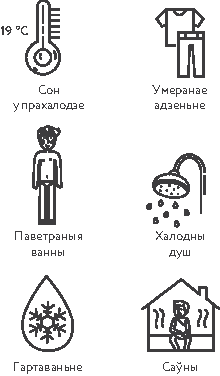
\includegraphics[scale=1.5]{willpower/ch12/5.pdf}
\end{figure}

\textbf{Сьвятло.} Лішак штучнага сьвятла ўвечары і ўначы можа блякаваць працу бурага тлушчу, гэтак жа як і ўжываньне бэта-блякатараў і дрэнная праца шчытавіцы. У дасьледаваньнях паказана, што ў~мышэй, якіх доўга трымалі на сьвятле, назапашвалася на 25--50\,\% больш тлушчу, хоць іх кармілі аднолькава. Чым сьвятлей у~вас у~спальні ўначы, тым вышэйшая рызыка атлусьценьня!

\textbf{Цеплавая працэдура.} Цеплавыя працэдуры ў~розных відах былі ва ўсіх старажытных цывілізацыях. У антычныя часы лазьні сталі сапраўднымі аздараўленчымі цэнтрамі з~гімнастычнымі залямі, парнымі, басэйнамі з~вадой розных тэмпэратураў, гразевымі ваннамі і масажам. Тэрмы Дыяклетыяна ў~Рыме зьмяшчалі да трох з~паловай тысячаў чалавек адначасова!

\emph{У «Аповесьці мінулых гадоў» ад асобы апостала Андрэя прыведзена апісаньне старажытнарускіх лазьняў: «Дзіўнае бачыў у~славянскай зямлі, калі ішоў сюды. Бачыў лазні драўляныя, і напаляць іх да чырвані, і распрануцца, і будуць голымі, і абальюцца квасам скураным, і ўзнімуць на сябе маладыя пруты, і б’юць сябе самі, і да таго даб’юцца, што вылезуць ледзь жывыя, і абальюцца вадою сцюдзёнаю, і так ажывуць. І тое твораць ва ўсе дні, ніхто ж іх не мучыць, але самі сябе мучаць, і гэтак твораць амавенне сабе, а~не пакуту».}

Цеплавы стрэс зьніжае рызыку сьмерці ад сардэчна-сасудзістых захворваньняў. Так, аматары саўнаў на 44\,\% радзей паміралі ад раптоўнага спыненьня сэрца, рызыка гіпэртэнзіі зьніжалася на 47\,\%. Дадатны эфэкт ёсьць таксама і для мозгу (зьніжэньне рызыкі Альцгаймэра і стымуляцыя нэўраплястычнасьці), для мэтабалізму (павелічэньне адчувальнасьці да інсуліну) і іншыя плюсы. Пры гэтым наведваньні 2--4 разы на тыдзень карысьнейшыя, чым раз на тыдзень. Цеплавы стрэс выклікае павелічэньне колькасьці бялкоў цеплавога шоку, якія дапамагаюць аднаўляць у~клетках пашкоджаныя малекулы.

Саўны і гарачыя ванны паляпшаюць кантроль глюкозы ў~крыві і нават зьмяншаюць колькасьць тлушчу, яны могуць быць карысныя для людзей з~цукроўкаю 2-га тыпу. Але яшчэ яны могуць нэгатыўна паўплываць на фэртыльнасьць мужчынаў (роўна як і занадта цёплая ніжняя бялізна, вузкія штаны, звычка трымаць ноўтбук на нагах і т. п.), бо павелічэньне тэмпэратуры ў~вобласьці машонкі парушае спэрматагенэз. Зрэшты, гэты ўплыў зварачальны.

\subsection*{Пытаньні і заданьні}

1. Сьпіце ў~прахалодзе.

2. Пачніце прымаць раніцай і ўвечары халодны ці кантрасны душ.

3. Схадзіце ў~саўну.


\section{Карысныя бактэрыі}

За дзесяць сэкундаў пацалунку пары абменьваюцца больш за 80 мільёнамі бактэрыяў, якія належаць да 150--300 відаў. У пастаянных партнёраў мікрафлёра рота наогул становіцца аднолькавай. Калі вы і ваш абраньнік/абраньніца здаровыя, то павелічэньне разнастайнасьці карысных бактэрыяў пойдзе вам абаім на карысьць.

Калі вы ясьце, ваша ежа корміць яшчэ й велізарнае мноства вашых малюсенькіх сяброў у~кішачніку~--- і тут гаворка таксама пра бактэрыі. Сяброўства зь імі забясьпечвае здароўе, а~сапсаваныя адносіны могуць нэгатыўна паўплываць на разьвіцьцё розных хваробаў~--- ад атлусьценьня і дэпрэсіі да алергій і харчовай непераноснасьці. Навукоўцы апісваюць ня толькі мікрабіем кішачніка, але й мікрабіёмы скуры, рота, дыхальных шляхоў, похвы і да т.~п.

У склад мікрабіёмы ўваходзяць ня толькі бактэрыі, але й вірусы, археі, найпрасьцейшыя і грыбы. У норме разнастайнасьць бактэрыяў дасягае 300--700 відаў мікраарганізмаў. Мікрабіёму нават называюць «другім геномам» і «другім мозгам», бо яна можа ўплываць на наша здароўе з~дапамогай мноства мэханізмаў. Нашы гены не памяняеш, а~вось на мікрафлёру часткова можна актыўна ўплываць. Даследаваньні паказваюць, што наша мікрафлёра дазваляе прадказваць наяўнасць шэрагу захворваньняў на 20\,\% дакладней, чым геном (за выключэннем дыябэту 1 тыпу). Рэч у~тым, што мікрабіём дакладней адлюстроўвае наш лад жыцьця, у~тым ліку гісторыю разьвіцьця, харчаваньне, фізычную актыўнасьць і інш.

\emph{Аналіз мікрабіёмы можа нават прадказаць рызыку сьмерці: наяўнасьць вялікай колькасьці бактэрыяў зь сямейства Enterobacteriaceae на 15\,\% павялічвае рызыку сьмерці на працягу бліжэйшых 15 гадоў.}

Калі ў~мікрабіёме больш патагенных штамаў, якія вылучаюць аміяк, індол, фэнол і да т.~п., то павялічваецца рызыка разьвіцьця дэмэнцыі. Прадказаць загостраньне недыху можна і па зьмене мікрабіёмы дыхальных шляхоў: чым вышэй узровень бактэрыяў Moraxella, Staphylococcus і чым ніжэй Corynebacterium, тым больш імавернасьць загостраньня. А на паверхні вачэй жыве карысная бактэрыя Corynebacterium mastitidis, якая стымулюе лякальны імунітэт і зьмяншае рызыку запаленьня і сьлепаты.

\textbf{Фармаваньне мікрафлёры} пачынаецца ўнутрычэраўна. Магчыма, некаторыя штамы могуць трапляць ужо на стадыі плоду, затым пры нараджэньні адбываецца масавае засяленьне нованароджаных бактэрыямі. Пасьля гэтага кантакт з~маці, грудное гадаваньне, асяродзьдзе~--- абсалютна ўсё ўплывае і кіруе засяленьнем кішачніка. У жаночым малаку ёсьць як бактэрыі, так і прэбіётыкі (алігацукрыды груднога малака), шмат розных злучэньняў, якія падтрымліваюць рост карысных бактэрыяў, такіх як біфідабактэрыі. Чым менш разнастайны мікрабіём у~маці і чым больш стэрыльнае асяродзьдзе, тым горшы будзе мікрабіём у~дзіцяці.

Варта адзначыць, што генэтыка амаль не ўплывае на склад мікрабіёму, асноўны ўклад уносіць менавіта асяродзьдзе. 

Рэзкія ўзьдзеяньні, такія як радыкальная зьмена дыеты альбо ўжываньне антыбіётыкаў, выклікаюць моцныя зьмены мікрафлёры кішачніка, але яны, як правіла, хутка зварачальныя. У кожнага чалавека ёсьць пастаянная, ядзерная мікрафлёра, якая мала мяняецца зь цягам часу.

\subsection*{Функцыі мікрафлёры}

Функцыі мікрафлёры вельмі разнастайныя і актыўна вывучаюцца апошнім часам. Мікрафлёра дапамагае падтрымліваць актыўнасьць імунітэту. Адэкватны мікрабіём абараняе кішачнік, канкуруючы са шкоднымі мікробамі і не даючы ім размнажацца, а~таксама падтрымлівае нармальную структуру кішачнага бар'ера, стымулюючы выпрацоўку сьлізі і пранікальнасьць. Бактэрыі дапамагаюць расшчапляць многія кампанэнты ежы і сынтэзаваць адсутныя (напрыклад, вітамін К і вітаміны групы В), уплываюць на ўсмоктваньне жалеза і кальцыю, інактывуюць многія біялягічна актыўныя малекулы. Мікрафлёра ўплывае і на артэрыяльны ціск. Калі звычайным пацукам перасадзіць мікрафлёру ад пацукоў-гіпэртонікаў, то ў~іх падымецца ціск. Дыета, багатая харчовымі валокнамі, акрамя ўсяго іншага, можа нават зьмяншаць артэрыяльны ціск! Склад мікрафлёры часта вызначае, як будуць для нас працаваць тыя ці іншыя лекі. 

\emph{Імунатэрапія раку больш эфэктыўная, калі ў~кішачніку ёсьць Akkermansia muciniphila. А выкарыстаньне антыбіётыкаў можа зьнізіць эфэктыўнасьць імунатэрапіі пухлінаў.}

\textbf{Уралітын.} Менавіта ад мікрафлёры залежыць, як на нас будуць уплываць пэўныя прадукты. Напрыклад, гранат будзе нашмат карысьнейшы тым людзям, чые бактэрыі ўмеюць утвараць з~яго уралітын-А, які валодае моцнымі ахоўнымі і супрацьзапаленчымі ўласьцівасьцямі. А вось наяўнасьць бактэрыяў Lactococcus garvieae, Lactobacillus mucosae, Bacteroides ovatus вызначае, ці будзе спажываньне соі ўплываць на зьніжэньне рызыкі раку грудзей, бо яна ўтварае S-эквал, які і вызначае гэты эфэкт.

\textbf{Трымэтыламінаксінд.} Часам бактэрыі ўтвараюць шкодныя злучэньні з~карысных кампанэнтаў ежы. Напрыклад, з~жывёльнай ежай у~арганізм паступаюць халін і карнітын. Мікрафлёра ўтварае з~іх трымэтыламінаксінд, высокі ўзровень якога зьвязаны з~больш высокай рызыкай (у 2,5 разы) разьвіцьця атэрасклерозу, інсульту і іншых сардэчна-сасудзістых захворваньняў. І што, няўжо мяса і яйкі так шкодзяць усім?! Аказалася, што ўзровень трымэтыламінаксінду вышэйшы, калі ў~мікрафлёры дэфіцыт карысных біфідабактэрыяў і шмат трымэтыламін-прадукавальных штамаў (Enterobacter, Acinetobacter, Proteus і інш.).

\emph{\textbf{Індол.} Пры расшчапленьні бялкоў у~кішачніку ўтворыцца шэраг прамежкавых злучэньняў, адзін зь іх~--- індол. З індолу розныя бактэрыі могуць сынтэзаваць шматлікія вытворныя: калі бактэрыі непрыязныя, то таксіны, а~іншыя могуць і карысныя злучэньні. Напрыклад, Clostridium sporogenes ператварае індол у~3-індолпрапіёнавую кіслату, якая зьяўляецца нэўрапратэктарам і антыаксідантам, а~таксама ўзмацняе бар'ерную функцыю кішачніка. Некаторыя віды Lactobacillus ператвараюць трыптафан у~індол-3-альдэгід, які дзейнічае на спэцыфічныя рэцэптары імунных клетак кішачніка і павялічвае выпрацоўку інтэрлейкіну-22.}

\textbf{Стрэс не заесьці.} Мікрафлёра ўплывае на настрой, таварыскасьць, узровень стрэсу і на вагу. Ведаючы склад мікрабіёты, можна з~дакладнасьцю да 90\,\% прадказаць атлусьценьне. Калі мікрафлёру ад тлустых мышэй перанесьці худым, то яны пачынаюць набіраць вагу, г.~зн. атлусьценьне можа быць заразным. Тыя, у~каго «набіраючая» мікрафлёра, маюць больш высокую рызыку атлусьценьня. Калі мы ямо шмат тлустага, нашы бактэрыі сынтэзуюць шмат ацэтату, які актывуе парасымпатыйную сыстэму, што выклікае ўзмоцненае выдзяленьне інсуліну і гармону голаду грэліну. А гэта можа зноў правакаваць пераяданьне.

Даданьне штаму Bifidobacterium infantis мышам у~стане стрэсу памяншала яго прыкметы і зьмяншала выяўленасьць дэпрэсіі і неспакою. Многія штамы Lactobacillus таксама дапамагаюць змагацца са стрэсам. Бактэрыя Bifidobacterium longum штам NCIMB 41676 зьніжае ўзровень картызолу, трывожнасьць і паляпшае памяць.

\infobox{Праца ў~садзе можа ўзбагаціць нас глебавымі бактэрыямі, напрыклад Mycobacterium vaccae, якія станоўча ўплываюць на настрой.}

\textbf{Віды штамаў.} Часта ўзьдзеяньне бактэрыі залежыць ад таго, які менавіта штам вас насяляе. Так, існуюць анкагенныя штамы Helicobacter pylori, якія павялічваюць рызыку раку страўніка, а~звычайныя яго штамы ў~страўніку могуць нават зьніжаць рызыку гастрыту і аўтаімунных захворваньняў. Бактэрыі сынтэзуюць з~харчовых валокнаў кароткаланцужковыя тлустыя кіслоты, якія моцна ўплываюць на ўвесь арганізм у~цэлым. Розныя тыпы бактэрыяў утвараюць ацэтат (воцатная кіслата), прапіянат (прапіёнавая кіслата) і найболей важны~--- бутырат (алейная кіслата). Ацэтат зьяўляецца крыніцай энэргіі, стымулюе маторыку і сакрэцыю кішачніка, валодае антымікробнымі эфэктамі. Прапіянат абараняе кішачнік ад патагенных мікраарганізмаў і ўдзельнічае ў~шэрагу біяхімічных рэакцый.

\textbf{Бутырат} падтрымлівае здароўе кішачніка: стымулюе абнаўленьне клетак сьлізістай, зьяўляецца для іх крыніцай энэргіі, стымулюе крывацёк і ўтварэньне сьлізістай, дае мноства іншых дабратворных эфэктаў, ад паляпшэньня працы мозгу да зьніжэньня запаленьня, рэгулюе актыўнасьць шэрагу генаў і можа падаўжаць жыцьцё. Бутырат таксама ўзмацняе нэўрагенэз у~мозгу, зьніжае верагоднасьць дэмэнцыі, паляпшае адчувальнасьць да інсуліну і дапамагае схуднець. Да бутырат-прадукавальных бактэрыяў адносяцца ў~асноўным роды Clostridium, Eubacterium і Butyrivibrio.

\subsection*{Пытаньні і заданьні}

1. Ці ёсьць у~вас праблемы са страваваньнем?

2. Ці часта вам прызначалі антыбіётыкі?

3. Вывучыце сваю мікрафлёру з~дапамогай аналізаў.


\section{Як палепшыць мікрафлёру}

Мы ведаем, што мікрабіём значна ўплывае на наша здароўе, але цяпер мала стандартаў і даведзеных спосабаў на яго радыкальна паўплываць. Чаму? Мікрабіём вельмі складаны, гэта сотні відаў, якія знаходзяцца ў~розных узаемадзеяньнях і падтрымліваюць сваю ўстойлівасьць. Таму мікрабіем супраціўляецца зьменам, а~нашы бактэрыі імкнуцца не дапусьціць пачаткоўцаў і пазбавіцца іх. На калянізацыю бактэрыяў уплываюць асаблівасьці імунітэту чалавека, стыль яго харчаваньня, прэпараты, якія ён прымае. Таксама варта памятаць, што ў~кожнага з~нас ёсьць базавая мікрафлёра, якая мала мяняецца на працягу жыцьця. Таму даданьне адной бактэрыі з~700 ці наўрад радыкальна паўплывае на здароўе кішачніка, асабліва калі мы ня ведаем, ці ёсьць у~нас яе недахоп.

Перадусім выконваць правілы падтрыманьня здаровага мікрабіёма: не забіваць бактэрыі (залішняе выкарыстаньне антыбіётыкаў, антысэптыкаў і да т.~п.), выконваць рэжым здаровага харчаваньня, стварыць багатае карыснымі мікраарганізмамі асяродзьдзе. Калі вы хочаце дзейнічаць больш выбарча, то патрэбныя дакладныя мэтады аналізу мікрабіёму. 

\textbf{Залаты стандарт~--- мэтагеномнае 16S рРНК-сэквэніраваньне, якое пакажа дакладны стан мікрабіёма і яго разнастайнасьць.}

\textbf{Разнастайнасьць мікрабіёма}~--- гэта першы і адзін з~найважнейшых паказьнікаў яго здароўя. Большая колькасьць розных відаў бактэрыяў забясьпечвае ім больш складаныя і збалянсаваныя адносіны адно з~адным і, як вынік, аптымальнае праходжаньне працэсаў страваваньня.

Звужэньне бактэрыяльнай разнастайнасьці~--- гэта кара нашага часу. Яно адбываецца кумулятыўна: чым меншая разнастайнасьць у~бацькоў, тым меншая будзе ў~іх дзяцей. Мы паступова губляем многія штамы бактэрыяў, якія былі ў~арганізьме людзей дзясяткі тысячаў гадоў. Паляпшэньне экалёгіі і апрацоўка ежы, выкарыстаньне мыйных сродкаў, антысэптыкаў, памяншэньне кантакту з~глебай, строгія санітарныя стандарты~--- усё гэта прыводзіць да драматычнага памяншэньня колькасьці бактэрыяў, якія маглі б узбагаціць нашу мікрафлёру. Памяншэньне разнастайнасьці харчаваньня і колькасьці расьліннай ежы ў~рацыёне, павелічэньне колькасьці мяса і тлушчу, рафінаваных прадуктаў, скарачэньне колькасьці харчовых валокнаў~--- усё гэта пазбаўляе нашу мікрафлёру харчаваньня, зьніжаючы яе разнастайнасьць.

\infobox{Чым меншая разнастайнасьць, тым горшая ўстойлівасьць добрых бактэрыяў да ўкараненьня чужародных і небясьпечных.}

\begin{figure}[htb!]
  \centering
  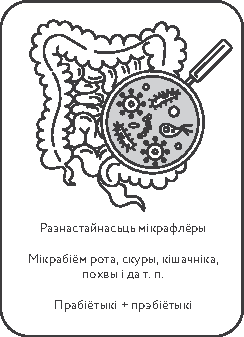
\includegraphics[scale=1.5]{willpower/ch12/6.pdf}
\end{figure}

\textbf{Ужываньне антыбіётыкаў} спустошвае мікрабіем, прычым нават аднаразовы курс можа прывесьці да зьніжэньня разнастайнасьці. Калі вы не ўжываеце антыбіётыкі для лячэньня, яны ўсё роўна могуць трапляць да вас у~арганізм зь мясам, яйкамі і малаком, бо 70\,\% антыбіётыкаў у~сусьветнай гаспадарцы вырабляецца для жывёлагадоўлі. Нэгатыўна ўзьдзейнічаць на мікрафлёру могуць і іншыя прэпараты, ад тых, што зьніжаюць кіслотнасьць страўніка, да антыдэпрэсантаў, а~таксама многія харчовыя дабаўкі, ад загушчальнікаў да цукразаменьнікаў. Лішак алькаголю, цукру, пераяданьне пагаршаюць склад мікрафлёры.

Мы звыклі да ідэі, што для паляпшэньня мікрафлёры трэба абавязкова нешта есьці. Аднак ёсьць гіпотэзы, што адной з~прычынаў парушэньняў зьяўляецца акурат лішак пажыўных рэчываў, і абмежаваньні ў~харчаваньні могуць палепшыць стан кішачніка.

На мікрафлёру дабратворна ўплывае ўмацаваньне іншых рэсурсаў здароўя, напрыклад дастатковы сон. Дэфіцыт сну спрыяе парушэньню суадносінаў паміж Firmicutes і Bacteriodetes, што зьяўляецца чыньнікам рызыкі атлусьценьня. Зь іншага боку, павелічэньне прадукцыі бутырату падаўжае фазу глыбокага сну і вядзе да ніжэйшых значэньняў тэмпэратуры цела. Фізычная актыўнасць паляпшае разнастайнасьць мікрафлёры і яе склад, але пры спыненьні заняткаў эфэкт хутка зьнікае. Сонечнае сьвятло таксама паляпшае мікрабіем: ультрафіялет спрыяе павелічэньню колькасьці бутырат-прадукавальных відаў бактэрый. Дадаткі вітаміну D могуць часткова ўзнавіць гэты эфэкт. Паляпшэньне працы імуннай сыстэмы, якое прыводзіць да павелічэньня выпрацоўкі супрацьзапаленчых цітакінаў, такіх як ІЛ-22, таксама дабратворна адбіваецца на складзе мікрабіёмы.

\textbf{Харчаваньне.} Здаровае харчаваньне падкормлівае добрую мікрафлёру, дрэннае~--- патагенныя штамы бактэрыяў. Некаторыя папулярныя дыеты, такія як карнівор ці кета, могуць прыводзіць да прыкметнага пагаршэньня мікрафлёры. Лішак тлушчу, цукру, алькаголю, пераяданьне, нерэгулярнае харчаваньне шкодзяць мікрафлёры. Пры нізкай разнастайнасьці мікрафлёры часьцей сустракаецца залішняя вага, інсулінарэзістэнтнасьць, ніжэй узровень ЛПВП, вышэй узровень трыгліцерыдаў, СЖК, лептыну і тп.

\emph{Дасьледаваньні мікрафлёры ў~блізьнятаў паказалі, што тыя зь іх, у~каго меншая разнастайнасьць мікрафлёры, маюць і большую вагу.}

Дастатковая колькасьць разнастайнай цэльнай умерана апрацаванай расьліннай ежы~--- адна з~найважнейшых умоваў падтрыманьня здаровай мікрафлёры. Тэрмічна апрацаваная гародніна ня горшая, а~часьцяком і лепшая за сырую для здароўя мікрафлёры. Памятайце і пра ўмеранасьць: чым больш і часьцей мы ямо, тым горшая ўзгодненасьць працы нашай мікрафлёры.

\textbf{Разнастайнасьць харчаваньня}~--- ключ да разнастайнасьці бактэрыяў. Адны віды бактэрыяў могуць есьці розныя валокны, а~некаторыя вельмі пераборлівыя. Павялічваючы колькасьць іх ``любімай'' ежы, мы павялічваем і іх канцэнтрацыю ў~страўніку. Напрыклад, бактэрыя Bacteroides thetaiotaomicron аддае перавагу гароху. Станоўча на мікрафлёру дзейнічаюць напоі: зялёная гарбата, какава, цукора. Напрыклад, эпігалакатэхін, які маецца ў~зялёнай гарбаце, павялічвае колькасьць бактэрыяў Flavonifractor plautii зь сямейства Clostridia, што могуць здымаць запаленьне і нават спрыяць зьніжэньню вагі. Яны прыгнятаюць імунны адказ Т-хэлпэраў на харчовыя алергены. Таксама зялёная гарбата спрыяе і росту іншых відаў карысных бактэрыяў.

Бабовыя ўтрымліваюць шмат харчовых валокнаў і дабратворна ўплываюць на мікрафлёру. Павелічэньне колькасьці гародніны (капуста, цыбуля, батат, гарбуз, бурак, артышок і да т.~п.), зеляніны, грыбоў, водарасьцяў, гарэхаў, садавіны, ягадаў забясьпечыць дастатковую колькасьць клятчаткі ды іншых прэбіётыкаў.

\infobox{Фастынг у~розных формах паляпшае мікрафлёру, павялічваючы колькасьць карысных бактэрыяў і зьмяншаючы аб'ём шкодных.}

\subsection*{Прэбіётыкі}

\textbf{Прэбіётыкі}~--- гэта розныя віды злучэньняў, якія служаць ежай для бактэрыяў і ня ўсмоктваюцца нашым арганізмам. Яны зьмяшчаюцца як у~цэльных прадуктах, так і ў~выглядзе дабавак. У цэлым я прыхільнік таго, каб атрымліваць іх з~прадуктамі, пагатоў гэта зусім не складана. Прэбіётыкаў шмат у~цэльным збожжы (цэльны авёс асабліва багаты), у~ім шмат як нераспушчальных харчовых валокнаў, так і распушчальных (бэта-глюкан). Прэбіятычны эфэкт маюць розныя алігацукрыды (напрыклад, фруктаалігацукрыды садавіны і ягадаў, галоктаалігацукрыды груднога малака, манан-алігацукрыды грыбоў), цукры (сарбіт, лактулоза), самыя розныя поліцукрыды (нераспушчальныя харчовыя валокны~--- цэлюлоза, лігнін, распушчальныя~--- геміцэлюлозы, глюканы, пэкціны, камедзь, карагенаны, рэзістэнтныя крухмалы, інулін, сьлізі і інш.) і шэраг іншых злучэньняў.

\emph{Напрыклад, рэзістэнтны крухмал~--- гэта разнавіднасьць крухмалу, устойлівага да перастраварваньня ў~тонкім кішачніку, што дзейнічае як прэбіётык. Ён маецца ў~бабовых, цэльных зернях, нясьпелых бананах, сырой бульбе, а~таксама астуджаным хлебе і збожжавых.}

\textbf{Харчовыя валокны} маюць шмат дадатных уласьцівасьцяў і не зьвязаных зь мікрафлёрай. Яны зьніжаюць рызыку запораў, памяншаюць глікемічны індэкс, хутчэй насычаюць і зьніжаюць рызыку пераяданьня. 30 грамаў клятчаткі памяншаюць на 20\,\% і больш рызыку сардэчна-сасудзістых захворваньняў, раку прамой кішкі і дыябэту, зьніжаюць сьмяротнасьць ад інфэкцыйных захворваньняў. Ніжняя мяжа нормы спажываньня харчовых валокнаў складае 30--35 грамаў, але паказьнік у~50 грамаў будзе больш аптымальным.

Самая высокая разнастайнасьць мікрафлёры ў~сучасным сьвеце ў~людзей з~плямёнаў паляўнічых-зьбіральнікаў, што абумоўлена ня толькі іх багатым бактэрыямі асяродзьдзем, але і вялікай колькасьцю зьяданых харчовых валокнаў, да 75--100 грам у~дзень. 30 грам клятчаткі памяншае на 20\,\% і больш рызыку сардэчна-сасудзістых захворваньняў, раку прамой кішкі і дыябэту, зьніжае сьмяротнасьць ад інфэкцыйных захворваньняў.

Зьвярніце ўвагу, што ў~складзе многіх прадуктаў больш за ўсё валокнаў у~лупіне ды іншых цьвёрдых частках, а~ня ў~мякаці. Таму перапрацаваныя і рафінаваныя прадукты, як правіла, утрымліваюць нашмат менш валокнаў. Павялічвайце колькасьць валокнаў паступова, бо рэзкае павелічэньне можа прывесьці да балючых адчуваньняў у~кішачніку. Пачніце не з~сырой, а~з тэрмічна апрацаванай гародніны, затым пераходзьце да альдэнтэ і толькі пасьля гэтага павелічайце колькасьць сырой.

\textbf{Прабіётыкі}~--- карысныя штамы жывых бактэрыяў, якія выкарыстоўваюцца ў~тэрапеўтычных мэтах. Зь імі цяпер склалася дастаткова парадаксальная сытуацыя. З аднаго боку, мы бачым рост зьвестак пра велізарны ўплыў мікрафлёры, можам дакладна даведацца індывідуальны склад мікрафлёры, але дагэтуль ня маем добрых якасных прэпаратаў, надзейных клінічных доказаў іх эфэктыўнасьці, дастатковых для фармаваньня выразнага кіраўніцтва да дзеяньня. З чым гэта можа быць зьвязана? Магчыма, прычыны~--- у~складанасьці мікрабіёмы, у~сотнях відаў мікраарганізмаў, якія ўзаемадзейнічаюць тысячамі спосабаў. Пры такой разнастайнасьці агульныя лінейныя падыходы не працуюць. Можа быць, уся справа ў~індывідуальных асаблівасьцях чалавека, бо амаль палова людзей рэзістэнтныя да прабіётыкаў~--- бактэрыі не засяляюць кішачнік.

\emph{Чакаем навінаў па стварэньні штамаў з~зададзенымі ўласьцівасьцямі, напрыклад, такіх, якія змогуць праграмаваць імунную сыстэму ўжо ў~дзяцінстве, і па стварэньні складаных збалянсаваных паміж сабой комплексаў прабіётыкаў. А пакуль варта сфакусавацца на павелічэньні разнастайнасьці мікрабіёма ў~цэлым, знаходзячы асаблівыя для гэтага падыходы.}

Шэраг дасьледаваньняў паказваюць эфэктыўнасьць прабіётыкаў, якія зьніжаюць частату дыярэі, паляпшаюць ліпідны профіль, зьніжаюць частату інфэкцыяў і г.~д. Але бязь зьмены харчаваньня прабіётыкі могуць і нашкодзіць. У адным з~дасьледаваньняў на жывёлах прабіятычныя бактэрыі пры нездаровым рацыёне праяўлялі патагенную актыўнасьць, а~вось у~групе здаровага харчаваньня паводзілі сябе бязь зьменаў. 

\infobox{Многія карысныя бактэрыі знаходзяцца ў~складзе фэрмэнтаваных прадуктаў, такіх як квас, кефір, ёгурт, а~таксама міса, кімчы і інш.}

Акрамя кішачніка, прабіётыкі могуць быць карысныя і для аднаўленьня і іншай мікрафлёры. Напрыклад, аральны прабіётык Streptococcus Salivarius штамы K12 (больш горла) і M18 (больш зубы), які зьніжае рызыку карыесу, танзілітаў ды іншых інфэкцыяў, пазбаўляе і ад непрыемнага паху з~рота і ўтварэньня камянёў. Lactobacillus sakei дапамагаюць аднавіць мікрафлёру насавых пазухаў, эфэктыўныя пры сінусіце. Ёсьць і прабіётыкі для скуры, напрыклад Streptococcus thermophiles у~выглядзе крэму павялічвае вытворчасьць ахоўных цэрамідаў, якія паляпшаюць бар'ерную функцыю скуры і маюць супрацьмікробныя ўласьцівасьці. Аднавіць мікрафлёру похвы і зьнізіць рызыку інфэкцыяў могуць штамы Lactobacillus crispatus CTV05, L. jensenii, ATCC 9857, L. gasseri, L. Iners, L. casei rhamnosus, L. acidophilus.

\emph{Якія прабіётыкі абраць? На ўпакоўцы звычайна пералічваюцца штамы, вось гэты сьпіс дапаможа вам абраць самыя эфэктыўныя. Лактабактэрыі: ужо апісаная Lactobacillus reuteri, Lactobacillus paracasei B 21060, L. rhamnosus GG, Lactobacillus casei DN114, Lactobacillus delbrueckii, L. plantarum W62, L. salivarius, Lactobacillus acido 052. Біфідабактэрыі: Bifidobacterium bifidum W23, B. lactis W18, B. longum W51, Bifidobacterium infantis, Bifidobacterium breve, Bifidobacterium animalis lactis. Энтэракокі: Enterococcus faecium W54. Бацылы: Bacillus clausii, Bacillus subtilis, Bacillus mesentericus. Стрэптакокі: Streptococcus faecalis, Streptococcus salivarius subsp. Thermophilius. Іншыя штамы: Pediococcus acidilactici CECT 7483, Clostridium butyricum і Escherichia coli DSM17252, E. coli Nissle 1917, Roseburia, Akkermansia Faecalibacterium prausnitzii. Грыбы Saccharomyces boulardii (сахараміцэтэты Булардзі) выкарыстоўваюцца пры лячэньні дыярэі і шэрагу іншых станаў.}

Хоць усе гэтыя штамы карысныя, эфэктыўнасьць іх паасобку не вялікая. Бо ў~кішачніку яны ўключаны ў~супольнасьці, дзе шчыльна ўзаемадзейнічаюць. Уявіце сабе завод па зборцы аўтамабіляў, дзе кожны працоўны робіць адну апэрацыю. Ці зможа замена аднаго працоўнага прыкметна павялічыць якасьць машынаў? Наўрад ці, важна зьмяняць усю сыстэму.

\emph{Таму і ёсьць такія мэтады лячэньня, як «супэрапрабіётык»~--- фэкальная трансплянтацыя (FMT Fecal microbiome transplantation) або перасадка калу, поўны перанос мікрабіёму ў~комплексе. У наш час перасадка калу можа дапамагчы пры розных праблемах: актыўна вывучаецца яе эфэктыўнасьць пры язвавым каліце, запорах, ляксах, інфэкцыях, сындроме раздражнёнага кішачніка і нават для лячэньня алькагольнай залежнасьці. Таксама цікавасьць уяўляюць і пазакішачныя захворваньні, такія як атлусьценьне, дыябэт, хвароба Паркінсана, аўтызм, расьсеянны склероз, дэпрэсія. Перасадка калу можа быць спосабам павысіць трывушчасьць. Так, бактэрыя Veillonella валодае здольнасьцю разбураць лактат, які назапашваецца падчас працяглых практыкаваньняў. Перасадка гэтай бактэрыі ў~мышэй на 13\,\% павялічвае іх трывушчасьць. Іншыя дасьледаваньні паказваюць, што перасадка калу ад больш трывушчых людзей на 6\,\% павялічвае сілу хвату на працягу месяца.}

Выкарыстоўваецца і перасадка мікрафлёры здаровае похвы, а~таксама ёсьць іншыя экспэрымэнтальныя спосабы. Напрыклад, пры кесаравым сячэньні абціраньне народжаных дзяцей тампонамі, уведзенымі ў~похву маці, паскарае іх засяленьне карыснымі штамамі Lactobacillus і Bacteroides. А біёляг Роберт Дан прапануе засяляць дамы карыснымі мікробамі, ствараць паверхні для размнажэньня дабратворных бактэрыяў.

\subsection*{Пытаньні і заданьні}

1. Пазьбягайце залішняга прымяненьня дэзінфэктантаў, антыбактэрыяльных мыйных сродкаў і да т.~п.

2. Забясьпечце сабе разнастайнае харчаваньне на аснове цэльнай расьліннай ежы.

3. Ежце дастатковую колькасьць харчовых валокнаў розных відаў.


\section{Больш добрых бактэрыяў вакол}

Санітарная рэвалюцыя рэзка зьнізіла колькасьць інфэкцыйных захворваньняў і перадухіліла вялікую колькасьць сьмерцяў ад іх. Але імкненьне максімальна скараціць прысутнасьць бактэрыяў, без падзелу на добрыя і дрэнныя, нараджае шмат новых праблемаў. Зьніжэньне разнастайнасьці бактэрыяў прыводзіць да зьніжэньня разнастайнасьці мікрафлёры кішачніка, што, у~сваю чаргу, вядзе да павелічэньня рызыкі алергій, аўтаімунных захворваньняў, харчовых алергій і т. д. Бо, рэагуючы на бактэрыі, імунітэт навучаецца і стрымлівацца, г.~зн. разьвіваецца яго супрацьзапаленчая актыўнасьць. Устаноўлена, што чым меншая мікробная экспазіцыя ў~дзяцінстве, тым вышэйы ў~дарослых узровень С-рэактыўнага бялку, а~значыць, і рызыка хваробаў, зьвязаных з~хранічным запаленьнем: дэпрэсія, дыябэт, раньняе старэньне, сардэчна-сасудзістыя захворваньні.

Рызыка алергій і аўтаімунных захворваньняў ніжэй у~вёсцы і вышэй у~гараджан. Сярод фэрмэраў іх менш у~тых, хто больш дапамагае бацькам з~жывёламі. А чым больш у~дзіцяці братоў і сясьцёр, тым меншая верагоднасьць разьвіцьця ў~яго алергічнага рыніту. Адны лекары лічаць, што алергіі~--- гэта непазьбежная плата за адсутнасьць інфэкцыйных хваробаў, а~іншыя прапаведуюць адмову ад гігіены для падтрыманьня здароўя.

Залатая сярэдзіна заключаецца ў~тым, каб строга выконваць правілы гігіены ў~небясьпечных месцах і сытуацыях, дзе можна выкарыстоўваць і антысэптыкі і антыбіётыкі. Напрыклад, пры сур'ёзнай інфэкцыі, а~таксама ў~аэрапорце, у~бальніцы, у~грамадзкіх месцах. Важна старанна сачыць і за санітарыяй ежы, мыць днушкі і да т.~п. Ніякай карысьці ў~кантакце са шкоднымі бактэрыямі няма. Залішняя чысьціня можа быць шкодная для вашай скуры, мы занадта часта і занадта моцна яе тром. Пастаянна змываючы ахоўны пласт тлушчу з~дапамогай мыйных сродкаў, мы толькі ўзмацняем актыўнасьць лоевых залоз, зьмяняецца кіслотнасьць нашай скуры, што спрыяе размнажэньню шкодных бактэрыяў. А калі мы змываем скурнае сала, гэта прыводзіць да сухасьці скуры і пазбаўляе ежы карысных скурных бактэрыяў. Адмова ад залішняй гігіены, як ні парадаксальна, можа палепшыць стан скуры і валасоў, і нават ваш пах. А вось мыць рукі (толькі не антыбактэрыйным мылам) важна больш старанна і рэгулярна, гэта сапраўды абараняе ад многіх захворваньняў.

\textbf{На прыродзе, дзе шмат карысных мікраарганізмаў, у~коле сваякоў, у~сябе дома імавернасьць прысутнасьці небясьпечных штамаў бактэрыяў мінімальная, таму залішнія намаганьні па выкананьні гігіены не патрэбныя.}

Напрыклад, ня трэба штодня прымаць душ з~мыйнымі сродкамі, калі ежа ўпала дома на падлогу, яе можна ўжываць. Нармальна цалавацца са здаровымі сваякамі. Нават калі дзіця выплёўвае пустышку на падлогу дома, мама можа проста яе аблізаць і вярнуць дзіцяці без кіпячэння. Дасьледаваньні выявілі, што такі спосаб зьвязаны з~меншай канцэнтрацыяй імунаглабуліну Е і рызыкай алергіі ў~дзяцей.

\emph{Гэта вельмі важна, бо з~самага нараджэньня вучыцца ня толькі нэрвовая сыстэма, але й імунная, і ў~іх абедзьвюх ёсьць крытычныя пэрыяды плястычнасьці. Нагадаю: калі раньняе дзяцінства праходзіць у~«паўстэрыльным асяродзьдзі», то імунная сыстэма не атрымлівае «адукацыю», што дае мноства праблемаў у~дарослага чалавека.}

Часьцей бываць на прыродзе, працаваць у~садзе, гуляць у~парках. Завесьці сабаку: у~сем'ях з~сабакамі дзеці радзей пакутуюць на алергіі ды аўтаімунныя захворваньні, у~іх большая разнастайнасьць мікрабіёма. Зразумела, павінен быць правільны догляд за сабакам, прышчэпкі і кантроль за глістамі. Падыдуць і іншыя жывёлы: чым больш зьвяроў і чым большыя яны па памеры, тым ніжэйшая рызыка алергій. Важна, каб такое ўзьдзеяньне было з~моманту нараджэньня. 

Спакойней стаўцеся да лёгкіх дзіцячых хваробаў. Бо перахварэўшы, дзіця часта становіцца ўстойлівейшым да шматлікіх хваробаў. Наведваньне гурткоў, садоў, зносіны з~аднагодкамі карысна для ўзбагачэньня мікрафлёры.

На працягу першых гадоў жыцьця імунная сыстэма дзіцяці праходзіць тонкую настройку, праграмуючыся пад узьдзеяньнем разнастайных антыгенаў. І калі нагрузка на імунную сыстэму недастатковая, то пажыцьцёва захоўваецца рызыка гіпэрактыўнасьці і хранічнага запаленьня, што прыкметна павышае рызыку алергічных, аўтаімунных захворваньняў і нават раку. У сем'ях, дзе ў~першыя пяць гадоў жыцьця былі хатнія жывёлы, колькасьць дзяцей-алергікаў аказалася рэзка зьніжаная. Такім чынам, здаровае бактэрыяльнае асяродзьдзе ўключае ў~сябе строгія меры па абароне ад шкоднасных інфэкцыяў і павелічэньне магчымасьцяў для кантакту з~карыснымі.

\subsection*{Пытаньні і заданьні}

1. Часьцей бывайце на прыродзе.

2. Кантактуйце з~жывёламі: каты, сабакі, коні і да т.~п.

3. Узбагачайце асяродзьдзе дзіцяці з~раньняга ўзросту.


\section{Візуальнае асяродзьдзе}

Прызнаюся, калі б ня стаў лекарам, то пайшоў бы ў~архітэктары: мяне захапляюць прыгожыя будынкі і дызайн. Біядызайн, на стыку архітэктуры і біялёгіі, цікавейшы за ўсё. Нядаўна на фэрмэрскім рынку ля дома купіў шмат гародніны і ў~чарговы раз дзівіўся капусьце раманэска. Структура раманэска фрактальная, г.~зн. «самападобная», калі яе драбнейшыя структуры паўтараюць буйнейшыя.

Фракталы вельмі распаўсюджаныя як у~жывой, так і нежывой прыродзе: аблокі, дрэвы, бранхіяльныя і сасудзістыя дрэвы, хвалі, лісьце расьлінаў, крыгі, лукавіны рэк, полымя вогнішча і да т.~п. Многія вонкава хаатычныя структуры маюць фрактальную будову, напрыклад, карціны Джэксана Полака. Натуральны ход пошукавых рухаў нашых вачэй~--- фрактальны. З аднаго боку, гэта самая эфэктыўная стратэгія пошуку, бо дазваляе пакрыць найбольшую адлегласьць, з~другога боку, мы выкарыстоўваем яе, магчыма, таму, што эвалюцыйна разглядалі фрактальныя аб'екты прыроды. 

Чым больш такіх структур у~навакольным асяродзьдзі, тым меншы ўзровень стрэсу вы адчуваеце і вам лягчэй увайсьці ў~стан «плыні». У дасьледаваньнях разгляданьне фрактальных структураў на экране вядзе да паляпшэньня стрэсаўстойлівасьці на 60\,\%. Пры разглядзе фракталаў у~лобнай кары павялічваецца альфа-актыўнасьць, пры гэтым дастаткова паглядзець усяго каля хвіліны. Дадайце больш фракталаў у~сваё жыцьцё, і гэта дапаможа вашай прэфранталцы лепш спраўляцца са стрэсам.

Выкарыстоўвайце біядызайн: глядзіце на аблокі, запаліце камін, пагуляйце на прыродзе. Азеляненьне, парк, лес, дрэвы~--- усё гэта вельмі дабратворна ўплывае на нас, фармуючы карыснае і аздараўленчае асяродзьдзе. Узровень азеляненьня~--- адзін з~надзейных, але дарагіх спосабаў падтрыманьня кагнітыўнага здароўя. Чым больш зеляніны, тым лепш разьвіцьцё мозгу ў~школьнікаў і тым павольней падзеньне кагнітыўных функцый у~старых. Азеляненьне на 15\,\% зьніжае рызыку нэўрадэгенэратыўных захворваньняў.

\infobox{Тут некалькі эфэктаў: просты візуальны антыстрэсавы эфэкт ад разглядваньня зеляніны, зьніжэньне паветранага забруджаньня, зьніжэньне роўню шуму, больш за ўмоваў для фізычнай актыўнасьці й ня толькі.}

\begin{figure}[htb!]
  \centering
  
\includegraphics[scale=1.5]{willpower/ch12/7.pdf}
\end{figure}

\textbf{Пагуляйце па лесе.} Дабратворны ўплыў прагулак па лесе або парку на стан здароўя чалавека пачаў вывучацца як навуковы фэномэн з~80-х гадоў XX стагодзьдзя. Калі раней людзі проста бралі заплечнік і сыходзілі ў~паход, цяпер прыдумалі больш адмысловых тэрмінаў. Першымі тут былі японцы, якія ўвялі тэрмін сінрын-ёку~--- ``лясныя ванны'', цяпер кажуць пра ``дэндратэрапію'', ``спа-лес'', Park Rx і інш. Можна выдатна спалучаць дзелавую сустрэчу, чытаньне або шпацыр з~дзецьмі ў~парку. Гэта станоўча ўзьдзейнічае на ваш мозг і ваша цела, не патрабуе напругі і заўсёды даступна.

\emph{Як заўважыў пісьменьнік Робэрт Стывэнсан, «Лес чаруе сэрцы людзей ня столькі сваёй прыгажосьцю, колькі цудоўным паветрам, эманацыяй старых дрэваў, нечым няўлоўным, што так цудоўна зьмяняе і аднаўляе стомлены дух».}

Устаноўлена, што прагулка па лесе на 15\,\% зьніжае ўзровень картызолу, на 4\,\% пульс і ціск, на 50\,\% павялічвае колькасьць NK-клетак у~крыві (натуральныя супрацьпухлінныя клеткі-кілеры), паляпшае імунную функцыю, зьніжае залішнюю актыўнасьць у~прэфрантальнай кары і ўзровень нэгатыўных эмоцыяў, зьніжае ўзровень глюкозы нават у~хворых на дыябэт, паляпшае працу вэгетатыўнай нэрвовай сістэмы.

\textbf{Глядзіце на аблокі.} Воблачная мэдытацыя~--- гэта ідэальная практыка. Аблокі прыгожыя і дзівосна чароўныя: ніколі ў~жыцьці мы ня бачым аднолькавых аблокаў, і кожны позірк у~неба ўнікальны. Заўважыць рух аблокаў і зьмена іх формы~--- ужо значыць досыць запаволіцца для рэляксацыі. Аблокі~--- гэта дафамін і крэатыўнасьць, калі мы знаходзім у~іх знаёмыя фігуры і падбіраем асацыяцыі. Гэта яшчэ і паднятая ўверх галава, што аўтаматычна паляпшае вашу паставу і настрой. З маіх любімых фракталаў~--- полымя, так расслабляе вогнішча на прыродзе або полымя каміна.

\textbf{Жывіце сярод прыгожай архітэктуры.} Амэрыканскі архітэктар Луіс Генры Салівэн сцьвярджаў, што ``Архітэктура~--- гэта мастацтва, якое ўзьдзейнічае на чалавека найбольш павольна, затое найбольш трывала''. Праблема дрэнных будынкаў таксама вельмі вялікая~--- яны вельмі павольна разбураюцца. 

Дасьледнікі хочуць ператварыць нешта няпэўнае~--- «фэнамэналёгію гарадзкой архітэктуры»~--- у~навуковыя факты нэўрабіялёгіі, вынікі якіх змогуць выкарыстоўваць дызайнэры і архітэктары. Навукоўцы ўпэўненыя, што «сузіральная архітэктура» можа зь цягам часу выклікаць такі ж карысны для здароўя эфэкт, што і мэдытацыя, але без намаганьняў чалавека.

Наш мозг насалоджваецца прапорцыямі, фракталамі і лініямі. Калі вы хочаце запаволіцца~--- знайдзіце самы прыўкрасны будынак у~вашым горадзе і дайце вачам магчымасьць атрымаць асалоду ад яго. Дасьледаваньне з~дапамогай МРТ дазволіла ўбачыць адрозьненьні ў~сузіраньні розных будынкаў і ацаніць мазгавы водгук на іх: разглядваньне архітэктурных шэдэўраў зьмяняе мэнтальнасьць чалавека, выклікаючы стан, блізкі да мэдытатыўнага. Чым больш у~будынку выкарыстана залатое сячэньне, тым лепш яно ўспрымаецца.

\textbf{Азеляняйце пакой.} Дасьледаваньні ўсталявалі, што хворым трэба менш абязбольвальных і яны хутчэй папраўляюцца, калі з~акна іх палаты відаць дрэвы. Пазьнейшыя працы паказалі, што дастаткова глядзець нават на фатаграфію прыроды. Разгляданьне жывых кветак расслабляе, зьніжае ўзровень стрэсу, павышае тонус антыстрэсавай парасімпатыйнай сыстэмы. Працуюць і асобныя элемэнты прыроднага асяродзьдзя: сьпевы птушак, расьліны, водары, гукі прыроды і г.~д. У зялёных офісах супрацоўнікі ня толькі лепей пачуваюцца, але й хутчэй прымаюць рашэньні. Фітадызайн дапаможа ўкараніць расьліны ў~ваша жыцьцё найболей зручным спосабам. Напрыклад, існуюць спэцыяльныя ``зялёныя сьцены'' з~аўтаматызаваным палівам. Калі не атрымліваецца хадзіць у~лес, можна зрабіць лес у~сябе дома!

\subsection*{Некамфортнае візуальнае асяродзьдзе}

Калі мы бачым нешта непрыемнае, то хочацца заплюшчыць вочы, каб паберагчы свае нэрвовыя клеткі. І гэта нядзіўна, бо тое, што мы бачым, уплывае на нашае здароўе. Прычым ня толькі ў~такога адчувальна віду, як чалавек,~--- нават у~мух.

\emph{Мухі рэагуюць на прысутнасьць мёртвых мух у~іх полі зроку. Нават пасіўная прысутнасьць мёртвых мух кароціць ім жыцьцё, а~вось даданьне антыдэпрэсанту перадухіляе заўчасную сьмерць.}

У сучасным горадзе мы бачым усё больш плоскіх паверхняў і прамых вуглоў. Мяняюцца колеры~--- меней зеляніны і болей шэрага, нас атачаюць машатбныя аднастайныя паверхні і багацьце тыпавых элемэнтаў. У прыродзе ж назіраецца велізарная колькасьць розных дэталяў, пры гэтым нельга знайсьці два аднолькавыя камені ці лісточкі.

\textbf{Агрэсіўнае асяродзьдзе.} Візуальнае асяродзьдзе, дзе шмат аднолькавых элемэнтаў, завецца агрэсіўным асяродзьдзем. Калі вы станеце тварам да шматпавярховага дома з~аднолькавымі панэлямі, то адчуеце, што на яго фізычна некамфортна глядзець. Рэч у~тым, што падчас глядзеньня нашы вочы робяць скокі, сакады. І калі пры пераскокваньні мы бачым адны і тыя ж дэталі, мозгу няма за што ўчапіцца, і ён змушаны павялічыць частату «скокаў». Разглядаючы старадаўнюю хату, мы кожны раз бачым розныя дэталі, і гэта нашмат камфортней для вачэй. 

\emph{Гамагенныя візуальныя асяродзьдзі~--- гэта асяродзьдзі, дзе вельмі мала прыкметных элемэнтаў, напрыклад, роўная белая сьцяна ці залітая асфальтам паркоўка або велізарныя паверхні пакрыцьцяў.}

Калі дадаць зеляніны, больш розных архітэктурных дэталяў, калярыстыкі і да т.~п. можна паменшыць агрэсію архітэктурнага асяродзьдзя. Прырода зьяўляецца ідэальным прыкладам камфортнага асяродзьдзя: лес, горы, аблокі~--- усё падпарадкоўваецца адзіным законам эстэтыкі. Акрамя задавальненьня, такое асяродзьдзе аптымальнае для нашай нэрвовай сыстэмы.

\subsection*{Пытаньні і заданьні}

1. Выбірайце для шпацыраў самыя прыгожыя маршруты.

2. Выкарыстоўвайце ў~дызайне дома элемэнты біядызайну. Карысныя нават фота і карціны прыроды.

3. Часьцей глядзіце на аблокі.


\section{Узбагачанае асяродзьдзе}

\begin{figure*}[htb!]
  \centering
  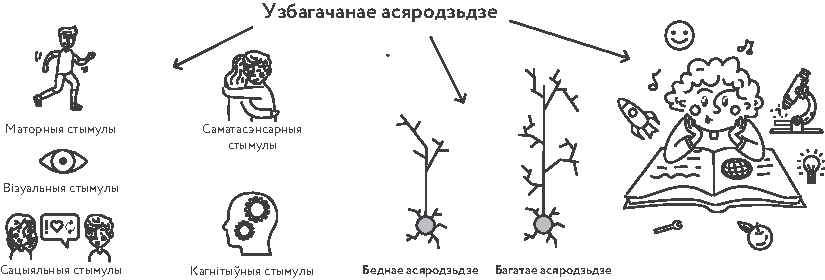
\includegraphics[scale=1.2]{willpower/ch12/8.pdf}
\end{figure*}

Калі пакласьці агурок у~расол, то ён стане салёным сам па сабе, без прымусу. Так і чалавек, зьмешчаны ва ўзбагачанае асяродзьдзе, становіцца разумнейшым, здаравейшым і жыве даўжэй, больш устойлівы да стрэсу. Узбагачанае асяродзьдзе~--- гэта адзін з~самых недаацэненых інструмэнтаў здароўя, у~тым ліку і грамадзкага.

\textbf{Узбагачанае асяродзьдзе}~--- гэта такое асяродзьдзе, дзе ў~вас ёсьць магчымасьць спантанных пошукавых паводзінаў, вялікая разнастайнасьць сродкаў задавальненьня базавых патрэбаў, актыўная сацыяльная падтрымка і магчымасьць усяляк сябе займаць, забаўляць і дасьледаваць. Магчыма многія з~вас краем вока бачылі такія дасьледаваньні, у~якіх адна група мышэй жыла ў~клетцы з~адной паілкай і кармушкай, а~другая група~--- у~клетцы, дзе былі колы для бегу, лазалкі, арэлі, прадметы з~рознай формай і да т.~п. Такое асяродзьдзе, дзе шмат розных стымулаў, і завецца ўзбагачаным. Пацукі ва ўзбагачаным асяродзьдзі жылі да 20\,\% даўжэй (аналяг~--- 90 чалавечых гадоў), мелі больш разьвіты мозг і колькасьць сінапсаў, былі больш худымі і мелі меншую рызыку раку. Чым складанейшыя псыхіка арганізма, тым мацней узьдзейнічае ўзбагачанае ці зьбедненае асяродзьдзе.

\textbf{Зьбедненае асяродзьдзе}~--- калі ёсьць эмацыйная, сэнсарная, рухальная дэпрывацыя, недахоп адпаведных уражаньняў. Жыцьцё ў~зьбедненым асяродзьдзі прыводзіць да разумовага адставаньня, неразьвітага маўленьня і парушэньняў рухальных навыкаў, павялічвае рызыку наркатычнай залежнасьці. На жаль, кампэнсаваць гэта ў~дарослых дастаткова цяжка.

\textbf{Узбагачанае асяродзьдзе} павялічвае колькасьць нэўратрафічных фактараў, што павялічвае нэўраплястычнасьць, устойлівасьць да стрэсу і выгараньня, кагнітыўныя здольнасьці, зьніжае рызыку нэўрадэгенэратыўных захворваньняў і да т.~п. Узбагачанае асяродзьдзе павялічвае памер мозгу, колькасьць нэўронаў і таўшчыню кары, памеры гіпакампа і ўзровень мазгавога нэўратрафічнага чыньніка, які стымулюе нэўраплястычнасьць BDNF. 

\textbf{Жывёлы і людзі ва ўзбагачаным асяродзьдзі хутчэй вучацца, лягчэй асвойваюць новыя навыкі, лягчэй даюць рады стрэсу.} 

\textbf{Паляпшэньне здароўя.} Цікава, што ўзбагачанае асяродзьдзе маці паскарае разьвіцьцё сятчаткі плода яшчэ ўнутрычэраўна. Дасьледаваньні паказалі, што ўзбагачанае асяродзьдзе паляпшае стан і навыкі дзяцей-аўтыстаў. Стымуляцыя тактыльная, пахавая, маторная пазітыўна адбівалася на іх стане. У дарослых узбагачанае асяродзьдзе паскарала рэабілітацыю пасьля інсульту.

Паказана станоўчае ўзьдзеяньне на розныя захворваньні, але самым уражлівым, на мой погляд, зьяўляецца зьніжэньне рызыкі разьвіцьця пухлінаў і запаволеньне іх росту. Вывучэньне ўзбагачанага асяродзьдзя пры гліёме паказала, што яно павышае выжывальнасьць, павышае актывацыю клетак імуннай сыстэмы макрафагаў і проціпухлінных NK-лімфацытаў. Сярод вывучаных відаў раку, узбагачанае асяродзьдзе дакладна эфэктыўны пры мэляноме, раку лёгкіх, падстраўніцы, грудзей, прамой кішкі. 

\infobox{Узбагачанае асяродзьдзе зьніжала памеры пухлінаў падстраўніцы розных відаў ад 41 да 53\,\%.}

Цікава, што дзеяньне ўзбагачанага асяродзьдзя комплекснае і ня зводзіцца толькі да аднаго зь яе чыньнікаў. Так, ізаляваная фізычная актыўнасьць хоць і паляпшала агульны стан, але нязначна ўплывала на рост пухлінаў. Асобна ўзятая сацыяльная актыўнасьць або толькі забаўкі ня мелі прыкметнага эфэкту. 

\textbf{Павелічэньне працягласьці жыцьця.} Жыць весела і доўга~--- што можа быць лепей? Самы вясёлы спосаб падаўжэньня жыцьця~--- праз стымуляцыю экспрэсіі дафамінавых Д2 рэцэптараў і стварэньне ўзбагачанага асяродзьдзя.

\emph{У экспэрымэнтах на мышах паказана, што мышы з~актыўным генам дафамінавага рэцэптара 2 тыпу ва ўмовах узбагачанага асяродзьдзя жылі на 22\,\% даўжэй, чым мышы без рэцэптара, а~вось проста актыўнасьць гена без асяродзьдзя не падаўжае жыцьця.} 

\textbf{Зьніжэньне рызыкі залежнасьці.} У дафамінавай сыстэме за нашу ўвагу канкуруюць розныя стымулы. Калі чалавек жыве ў~зьбедненым асяродзьдзі, то ён мае высокую рызыку хімічных і нехімічных залежнасьцяў, становіцца ўразьлівым. Стварэньне асяродзьдзя зьмяншае спажываньне наркотыкаў і аслабляе іншыя віды залежнасьцяў. Жыцьцё ў~зьбедненым асяродзьдзі прыводзіць да разумовага адставаньня, неразьвітага маўленьня і парушэньняў рухальных навыкаў, павялічвае рызыку наркатычнай залежнасьці. На жаль, кампэнсаваць гэта ў~дарослых дастаткова цяжка.

\subsection*{Стварыце або знайдзіце ўзбагачанае асяродзьдзе}

Каб чалавек узаемадзейнічаў з~элемэнтамі навакольнага асяродзьдзя, яны павінны быць для яго эмацыйна значнымі, цікавымі, а~таксама разнастайнымі, дынамічнымі. Важныя магчымасьць выбіраць, а~таксама авалодваць новымі навыкамі, атрымліваць новы досьвед і зваротную сувязь, пашыраць свае магчымасьці і самае важнае~--- пераўтвараць і ўзбагачаць асяродзьдзе асабіста. Вядома, пры гэтым важны і пэўны ўзровень стрэсу і непрадказальнасьці, што паляпшае навучаньне, але з~падтрыманьнем псыхалягічнай бясьпекі. 

\textbf{Візуальныя стымулы}: багатае візуальнае асяродзьдзе, а~ня шэры бетон панэлек-калюмбарыяў. 

\textbf{Сацыяльныя стымулы}: статус, падтрымка, устойлівыя сацыяльныя сувязі, а~ня сацыяльная ізаляцыя і адзінота. 

\textbf{Маторныя стымулы}: рухальнае навучаньне, разнастайная фізычная актыўнасьць, а~не сядзеньне па 12 гадзінаў у~дзень на крэсьле. 

\textbf{Саматасэнсарныя стымулы}: дотыкі, масаж, спорт, тэмпэратурныя ўзьдзеяньні, а~не ўвесьчасны цялесны камфорт.

\textbf{Кагнітыўныя стымулы}: задачы, выклікі, а~не манатонная праца.

Прадумайце магчымасьць харчовай разнастайнасьці, каштуйце новыя смакі, прадукты. Паспрабуйце розныя віды актыўнасьці, асвойце новыя рухальныя навыкі~--- танец або катаньне на роліках. Пашырце сфэру сваіх знаёмстваў, зьезьдзіце ў~новае месца, вазьміцеся за рашэньне нязвыклай задачы. Заўважана, што ідэі ўзьнікаюць у~пэўных колах, а~не паасобку. Дзе ўзбагачанае асяродзьдзе для вашых мэтаў?

\subsection*{Пытаньні і заданьні}

1. Дзе ля вас ёсьць асяродзьдзе, якое адпавядае вызначэньню ўзбагачанага асяродзьдзя?

2. Якія элемэнты ўзбагачанага асяродзьдзя вы можаце ўкараніць у~сябе дома?

3. Трэніруйце свой мозг гульнёй: паежце з~заплюшчанымі вачыма, разьвівайце нюх у~парфумэрнай краме або квяцярні, развучыце новы танец або верш на памяць.

\clearpage
\thispagestyle{empty}
\begin{figure}[htb!]
  \vspace*{-0.5in}
  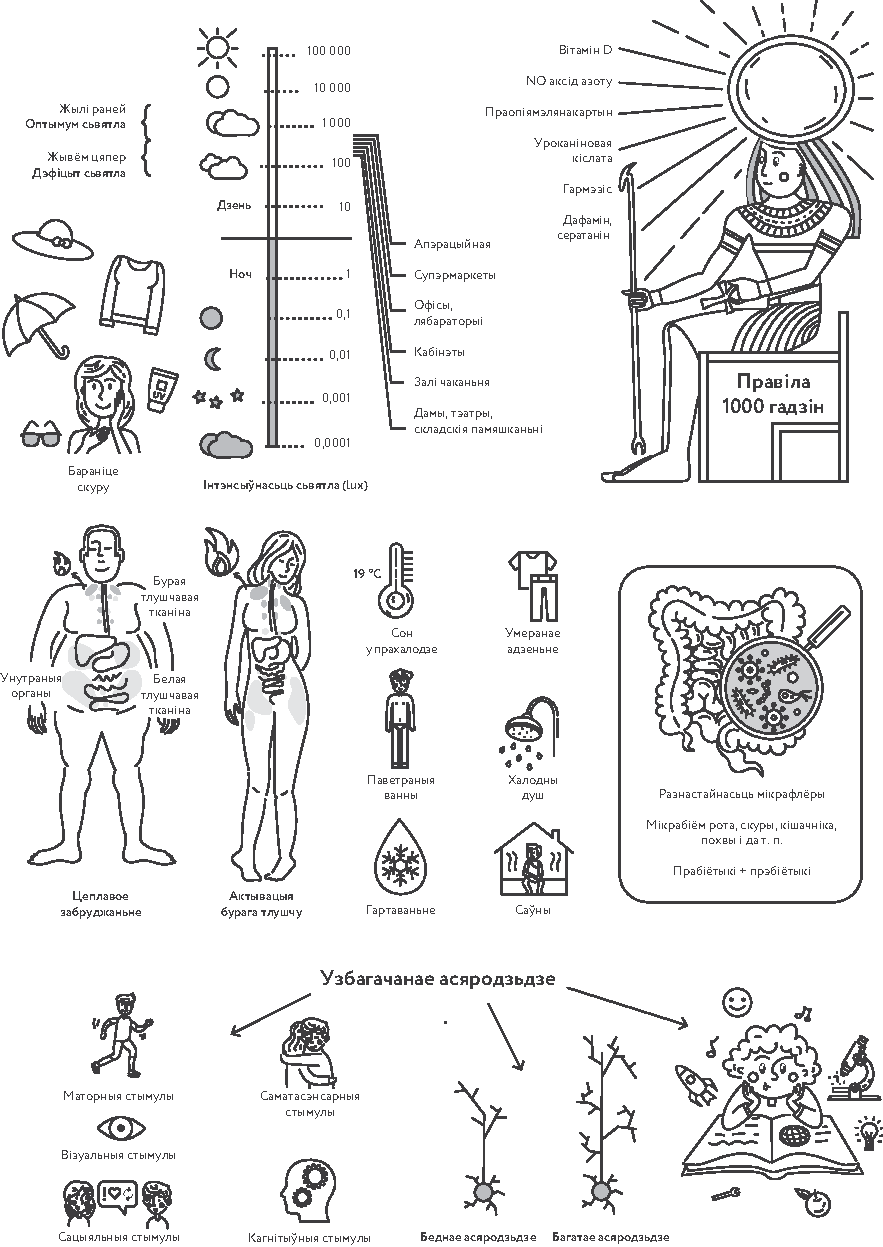
\includegraphics[width=\textwidth]{willpower/ch12/full.pdf}  
\end{figure}
